\documentclass[twoside]{book}

% Packages required by doxygen
\usepackage{fixltx2e}
\usepackage{calc}
\usepackage{doxygen}
\usepackage[export]{adjustbox} % also loads graphicx
\usepackage{graphicx}
\usepackage[utf8]{inputenc}
\usepackage{makeidx}
\usepackage{multicol}
\usepackage{multirow}
\PassOptionsToPackage{warn}{textcomp}
\usepackage{textcomp}
\usepackage[nointegrals]{wasysym}
\usepackage[table]{xcolor}

% Font selection
\usepackage[T1]{fontenc}
\usepackage[scaled=.90]{helvet}
\usepackage{courier}
\usepackage{amssymb}
\usepackage{sectsty}
\renewcommand{\familydefault}{\sfdefault}
\allsectionsfont{%
  \fontseries{bc}\selectfont%
  \color{darkgray}%
}
\renewcommand{\DoxyLabelFont}{%
  \fontseries{bc}\selectfont%
  \color{darkgray}%
}
\newcommand{\+}{\discretionary{\mbox{\scriptsize$\hookleftarrow$}}{}{}}

% Page & text layout
\usepackage{geometry}
\geometry{%
  a4paper,%
  top=2.5cm,%
  bottom=2.5cm,%
  left=2.5cm,%
  right=2.5cm%
}
\tolerance=750
\hfuzz=15pt
\hbadness=750
\setlength{\emergencystretch}{15pt}
\setlength{\parindent}{0cm}
\setlength{\parskip}{3ex plus 2ex minus 2ex}
\makeatletter
\renewcommand{\paragraph}{%
  \@startsection{paragraph}{4}{0ex}{-1.0ex}{1.0ex}{%
    \normalfont\normalsize\bfseries\SS@parafont%
  }%
}
\renewcommand{\subparagraph}{%
  \@startsection{subparagraph}{5}{0ex}{-1.0ex}{1.0ex}{%
    \normalfont\normalsize\bfseries\SS@subparafont%
  }%
}
\makeatother

% Headers & footers
\usepackage{fancyhdr}
\pagestyle{fancyplain}
\fancyhead[LE]{\fancyplain{}{\bfseries\thepage}}
\fancyhead[CE]{\fancyplain{}{}}
\fancyhead[RE]{\fancyplain{}{\bfseries\leftmark}}
\fancyhead[LO]{\fancyplain{}{\bfseries\rightmark}}
\fancyhead[CO]{\fancyplain{}{}}
\fancyhead[RO]{\fancyplain{}{\bfseries\thepage}}
\fancyfoot[LE]{\fancyplain{}{}}
\fancyfoot[CE]{\fancyplain{}{}}
\fancyfoot[RE]{\fancyplain{}{\bfseries\scriptsize Generated by Doxygen }}
\fancyfoot[LO]{\fancyplain{}{\bfseries\scriptsize Generated by Doxygen }}
\fancyfoot[CO]{\fancyplain{}{}}
\fancyfoot[RO]{\fancyplain{}{}}
\renewcommand{\footrulewidth}{0.4pt}
\renewcommand{\chaptermark}[1]{%
  \markboth{#1}{}%
}
\renewcommand{\sectionmark}[1]{%
  \markright{\thesection\ #1}%
}

% Indices & bibliography
\usepackage{natbib}
\usepackage[titles]{tocloft}
\setcounter{tocdepth}{3}
\setcounter{secnumdepth}{5}
\makeindex

% Hyperlinks (required, but should be loaded last)
\usepackage{ifpdf}
\ifpdf
  \usepackage[pdftex,pagebackref=true]{hyperref}
\else
  \usepackage[ps2pdf,pagebackref=true]{hyperref}
\fi
\hypersetup{%
  colorlinks=true,%
  linkcolor=blue,%
  citecolor=blue,%
  unicode%
}

% Custom commands
\newcommand{\clearemptydoublepage}{%
  \newpage{\pagestyle{empty}\cleardoublepage}%
}

\usepackage{caption}
\captionsetup{labelsep=space,justification=centering,font={bf},singlelinecheck=off,skip=4pt,position=top}

%===== C O N T E N T S =====

\begin{document}

% Titlepage & ToC
\hypersetup{pageanchor=false,
             bookmarksnumbered=true,
             pdfencoding=unicode
            }
\pagenumbering{roman}
\begin{titlepage}
\vspace*{7cm}
\begin{center}%
{\Large My Project }\\
\vspace*{1cm}
{\large Generated by Doxygen 1.8.11}\\
\end{center}
\end{titlepage}
\clearemptydoublepage
\tableofcontents
\clearemptydoublepage
\pagenumbering{arabic}
\hypersetup{pageanchor=true}

%--- Begin generated contents ---
\chapter{Namespace Index}
\section{Namespace List}
Here is a list of all namespaces with brief descriptions\+:\begin{DoxyCompactList}
\item\contentsline{section}{\hyperlink{namespacelySLAM}{ly\+S\+L\+AM} }{\pageref{namespacelySLAM}}{}
\item\contentsline{section}{\hyperlink{namespaceORB__SLAM2}{O\+R\+B\+\_\+\+S\+L\+A\+M2} }{\pageref{namespaceORB__SLAM2}}{}
\end{DoxyCompactList}

\chapter{Hierarchical Index}
\section{Class Hierarchy}
This inheritance list is sorted roughly, but not completely, alphabetically\+:\begin{DoxyCompactList}
\item \contentsline{section}{Mat\+Allocator}{\pageref{classMatAllocator}}{}
\begin{DoxyCompactList}
\item \contentsline{section}{ly\+S\+L\+AM\+:\+:Numpy\+Allocator}{\pageref{classlySLAM_1_1NumpyAllocator}}{}
\end{DoxyCompactList}
\item \contentsline{section}{ly\+S\+L\+AM\+:\+:Py\+Allow\+Threads}{\pageref{classlySLAM_1_1PyAllowThreads}}{}
\item \contentsline{section}{ly\+S\+L\+AM\+:\+:Py\+Ensure\+G\+IL}{\pageref{classlySLAM_1_1PyEnsureGIL}}{}
\end{DoxyCompactList}

\chapter{Class Index}
\section{Class List}
Here are the classes, structs, unions and interfaces with brief descriptions\+:\begin{DoxyCompactList}
\item\contentsline{section}{\hyperlink{classMatAllocator}{Mat\+Allocator} }{\pageref{classMatAllocator}}{}
\item\contentsline{section}{\hyperlink{classlySLAM_1_1NumpyAllocator}{ly\+S\+L\+A\+M\+::\+Numpy\+Allocator} }{\pageref{classlySLAM_1_1NumpyAllocator}}{}
\item\contentsline{section}{\hyperlink{classlySLAM_1_1PyAllowThreads}{ly\+S\+L\+A\+M\+::\+Py\+Allow\+Threads} }{\pageref{classlySLAM_1_1PyAllowThreads}}{}
\item\contentsline{section}{\hyperlink{classlySLAM_1_1PyEnsureGIL}{ly\+S\+L\+A\+M\+::\+Py\+Ensure\+G\+IL} }{\pageref{classlySLAM_1_1PyEnsureGIL}}{}
\end{DoxyCompactList}

\chapter{File Index}
\section{File List}
Here is a list of all files with brief descriptions\+:\begin{DoxyCompactList}
\item\contentsline{section}{\hyperlink{Conversion_8cc}{Conversion.\+cc} }{\pageref{Conversion_8cc}}{}
\item\contentsline{section}{\hyperlink{Converter_8cc}{Converter.\+cc} }{\pageref{Converter_8cc}}{}
\item\contentsline{section}{\hyperlink{Frame_8cc}{Frame.\+cc} }{\pageref{Frame_8cc}}{}
\item\contentsline{section}{\hyperlink{FrameDrawer_8cc}{Frame\+Drawer.\+cc} }{\pageref{FrameDrawer_8cc}}{}
\item\contentsline{section}{\hyperlink{Geometry_8cc}{Geometry.\+cc} }{\pageref{Geometry_8cc}}{}
\item\contentsline{section}{\hyperlink{Initializer_8cc}{Initializer.\+cc} }{\pageref{Initializer_8cc}}{}
\item\contentsline{section}{\hyperlink{KeyFrame_8cc}{Key\+Frame.\+cc} }{\pageref{KeyFrame_8cc}}{}
\item\contentsline{section}{\hyperlink{KeyFrameDatabase_8cc}{Key\+Frame\+Database.\+cc} }{\pageref{KeyFrameDatabase_8cc}}{}
\item\contentsline{section}{\hyperlink{LocalMapping_8cc}{Local\+Mapping.\+cc} }{\pageref{LocalMapping_8cc}}{}
\item\contentsline{section}{\hyperlink{LoopClosing_8cc}{Loop\+Closing.\+cc} }{\pageref{LoopClosing_8cc}}{}
\item\contentsline{section}{\hyperlink{Map_8cc}{Map.\+cc} }{\pageref{Map_8cc}}{}
\item\contentsline{section}{\hyperlink{MapDrawer_8cc}{Map\+Drawer.\+cc} }{\pageref{MapDrawer_8cc}}{}
\item\contentsline{section}{\hyperlink{MapPoint_8cc}{Map\+Point.\+cc} }{\pageref{MapPoint_8cc}}{}
\item\contentsline{section}{\hyperlink{MaskNet_8cc}{Mask\+Net.\+cc} }{\pageref{MaskNet_8cc}}{}
\item\contentsline{section}{\hyperlink{MaskNetStereo_8cc}{Mask\+Net\+Stereo.\+cc} }{\pageref{MaskNetStereo_8cc}}{}
\item\contentsline{section}{\hyperlink{Optimizer_8cc}{Optimizer.\+cc} }{\pageref{Optimizer_8cc}}{}
\item\contentsline{section}{\hyperlink{ORBextractor_8cc}{O\+R\+Bextractor.\+cc} }{\pageref{ORBextractor_8cc}}{}
\item\contentsline{section}{\hyperlink{ORBmatcher_8cc}{O\+R\+Bmatcher.\+cc} }{\pageref{ORBmatcher_8cc}}{}
\item\contentsline{section}{\hyperlink{PnPsolver_8cc}{Pn\+Psolver.\+cc} }{\pageref{PnPsolver_8cc}}{}
\item\contentsline{section}{\hyperlink{RegionProps_8cc}{Region\+Props.\+cc} }{\pageref{RegionProps_8cc}}{}
\item\contentsline{section}{\hyperlink{Semantic_8cc}{Semantic.\+cc} }{\pageref{Semantic_8cc}}{}
\item\contentsline{section}{\hyperlink{Sim3Solver_8cc}{Sim3\+Solver.\+cc} }{\pageref{Sim3Solver_8cc}}{}
\item\contentsline{section}{\hyperlink{SlamConfig_8cc}{Slam\+Config.\+cc} }{\pageref{SlamConfig_8cc}}{}
\item\contentsline{section}{\hyperlink{System_8cc}{System.\+cc} }{\pageref{System_8cc}}{}
\item\contentsline{section}{\hyperlink{Tracking_8cc}{Tracking.\+cc} }{\pageref{Tracking_8cc}}{}
\item\contentsline{section}{\hyperlink{Viewer_8cc}{Viewer.\+cc} }{\pageref{Viewer_8cc}}{}
\end{DoxyCompactList}

\chapter{Namespace Documentation}
\hypertarget{namespacelySLAM}{}\section{ly\+S\+L\+AM Namespace Reference}
\label{namespacelySLAM}\index{ly\+S\+L\+AM@{ly\+S\+L\+AM}}
\subsection*{Classes}
\begin{DoxyCompactItemize}
\item 
class \hyperlink{classlySLAM_1_1NumpyAllocator}{Numpy\+Allocator}
\item 
class \hyperlink{classlySLAM_1_1PyAllowThreads}{Py\+Allow\+Threads}
\item 
class \hyperlink{classlySLAM_1_1PyEnsureGIL}{Py\+Ensure\+G\+IL}
\end{DoxyCompactItemize}
\subsection*{Functions}
\begin{DoxyCompactItemize}
\item 
static void \hyperlink{namespacelySLAM_a00b314520d011d12b2bd631293ea02a8}{init} ()
\item 
static int \hyperlink{namespacelySLAM_a7b41c0e11cbb97ca1485abd44d51e799}{failmsg} (const char $\ast$fmt,...)
\item 
static Py\+Object $\ast$ \hyperlink{namespacelySLAM_a4c4e113b266fb98524f7c06154fe33e1}{failmsgp} (const char $\ast$fmt,...)
\item 
float \hyperlink{namespacelySLAM_a432cf91e1b1dee06c5d9a35cc1b5529a}{Area} (float x1, float x2, float y1, float y2)
\item 
void \hyperlink{namespacelySLAM_a83245374bbce9e47c4878b5613fb98db}{tic\+\_\+initsv} ()
\item 
void \hyperlink{namespacelySLAM_adb77bc91beb203170ca5a301968f9f76}{toc\+\_\+finalsv} (double \&time)
\item 
void \hyperlink{namespacelySLAM_af18d8f81de160c1de261c5465c29523e}{ticsv} ()
\item 
void \hyperlink{namespacelySLAM_a56e5af1fe2c6086f5597b0e44465ffc3}{tocsv} ()
\end{DoxyCompactItemize}
\subsection*{Variables}
\begin{DoxyCompactItemize}
\item 
\hyperlink{classlySLAM_1_1NumpyAllocator}{Numpy\+Allocator} \hyperlink{namespacelySLAM_a487059d3e4df5c492791c26d6316a9f2}{g\+\_\+numpy\+Allocator}
\item 
struct timeval \hyperlink{namespacelySLAM_a823e029c6b9b89870dc987acb8e9c032}{tvsv}
\item 
double \hyperlink{namespacelySLAM_ab1de636cddc68247bbed233099d643f9}{t1sv}
\item 
double \hyperlink{namespacelySLAM_a6b5e057f8ce421fbc6d49a07ef7e3273}{t2sv}
\item 
double \hyperlink{namespacelySLAM_aee2bcc68912513a06dfc54c894ae3efc}{t0sv}
\item 
double \hyperlink{namespacelySLAM_a76440f183e00c79997868ddfe1dae982}{t3sv}
\end{DoxyCompactItemize}


\subsection{Detailed Description}
This file is part of Dyna\+S\+L\+AM. Copyright (C) 2018 Berta Bescos $<$bbescos at=\char`\"{}\char`\"{} unizar=\char`\"{}\char`\"{} dot=\char`\"{}\char`\"{} es$>$=\char`\"{}\char`\"{}$>$ (University of Zaragoza) For more information see \href{https://github.com/bertabescos/DynaSLAM}{\tt https\+://github.\+com/bertabescos/\+Dyna\+S\+L\+AM}. 

\subsection{Function Documentation}
\index{ly\+S\+L\+AM@{ly\+S\+L\+AM}!Area@{Area}}
\index{Area@{Area}!ly\+S\+L\+AM@{ly\+S\+L\+AM}}
\subsubsection[{\texorpdfstring{Area(float x1, float x2, float y1, float y2)}{Area(float x1, float x2, float y1, float y2)}}]{\setlength{\rightskip}{0pt plus 5cm}float ly\+S\+L\+A\+M\+::\+Area (
\begin{DoxyParamCaption}
\item[{float}]{x1, }
\item[{float}]{x2, }
\item[{float}]{y1, }
\item[{float}]{y2}
\end{DoxyParamCaption}
)}\hypertarget{namespacelySLAM_a432cf91e1b1dee06c5d9a35cc1b5529a}{}\label{namespacelySLAM_a432cf91e1b1dee06c5d9a35cc1b5529a}


Definition at line 468 of file Geometry.\+cc.


\begin{DoxyCode}
468                                                   \{
469     \textcolor{keywordtype}{float} xc1 = max(x1-0.5,x2-0.5);
470     \textcolor{keywordtype}{float} xc2 = min(x1+0.5,x2+0.5);
471     \textcolor{keywordtype}{float} yc1 = max(y1-0.5,y2-0.5);
472     \textcolor{keywordtype}{float} yc2 = min(y1+0.5,y2+0.5);
473     \textcolor{keywordflow}{return} (xc2-xc1)*(yc2-yc1);
474 \}
\end{DoxyCode}
\index{ly\+S\+L\+AM@{ly\+S\+L\+AM}!failmsg@{failmsg}}
\index{failmsg@{failmsg}!ly\+S\+L\+AM@{ly\+S\+L\+AM}}
\subsubsection[{\texorpdfstring{failmsg(const char $\ast$fmt,...)}{failmsg(const char *fmt,...)}}]{\setlength{\rightskip}{0pt plus 5cm}static int ly\+S\+L\+A\+M\+::failmsg (
\begin{DoxyParamCaption}
\item[{const char $\ast$}]{fmt, }
\item[{}]{...}
\end{DoxyParamCaption}
)\hspace{0.3cm}{\ttfamily [static]}}\hypertarget{namespacelySLAM_a7b41c0e11cbb97ca1485abd44d51e799}{}\label{namespacelySLAM_a7b41c0e11cbb97ca1485abd44d51e799}


Definition at line 21 of file Conversion.\+cc.


\begin{DoxyCode}
22 \{
23     \textcolor{keywordtype}{char} str[1000];
24 
25     va\_list ap;
26     va\_start(ap, fmt);
27     vsnprintf(str, \textcolor{keyword}{sizeof}(str), fmt, ap);
28     va\_end(ap);
29 
30     PyErr\_SetString(PyExc\_TypeError, str);
31     \textcolor{keywordflow}{return} 0;
32 \}
\end{DoxyCode}
\index{ly\+S\+L\+AM@{ly\+S\+L\+AM}!failmsgp@{failmsgp}}
\index{failmsgp@{failmsgp}!ly\+S\+L\+AM@{ly\+S\+L\+AM}}
\subsubsection[{\texorpdfstring{failmsgp(const char $\ast$fmt,...)}{failmsgp(const char *fmt,...)}}]{\setlength{\rightskip}{0pt plus 5cm}static Py\+Object$\ast$ ly\+S\+L\+A\+M\+::failmsgp (
\begin{DoxyParamCaption}
\item[{const char $\ast$}]{fmt, }
\item[{}]{...}
\end{DoxyParamCaption}
)\hspace{0.3cm}{\ttfamily [static]}}\hypertarget{namespacelySLAM_a4c4e113b266fb98524f7c06154fe33e1}{}\label{namespacelySLAM_a4c4e113b266fb98524f7c06154fe33e1}


Definition at line 61 of file Conversion.\+cc.


\begin{DoxyCode}
62 \{
63     \textcolor{keywordtype}{char} str[1000];
64 
65     va\_list ap;
66     va\_start(ap, fmt);
67     vsnprintf(str, \textcolor{keyword}{sizeof}(str), fmt, ap);
68     va\_end(ap);
69 
70     PyErr\_SetString(PyExc\_TypeError, str);
71     \textcolor{keywordflow}{return} 0;
72 \}
\end{DoxyCode}
\index{ly\+S\+L\+AM@{ly\+S\+L\+AM}!init@{init}}
\index{init@{init}!ly\+S\+L\+AM@{ly\+S\+L\+AM}}
\subsubsection[{\texorpdfstring{init()}{init()}}]{\setlength{\rightskip}{0pt plus 5cm}void ly\+S\+L\+A\+M\+::\+N\+D\+Array\+Converter\+::init (
\begin{DoxyParamCaption}
{}
\end{DoxyParamCaption}
)\hspace{0.3cm}{\ttfamily [static]}}\hypertarget{namespacelySLAM_a00b314520d011d12b2bd631293ea02a8}{}\label{namespacelySLAM_a00b314520d011d12b2bd631293ea02a8}


Definition at line 16 of file Conversion.\+cc.


\begin{DoxyCode}
17 \{
18     import\_array();
19 \}
\end{DoxyCode}
\index{ly\+S\+L\+AM@{ly\+S\+L\+AM}!tic\+\_\+initsv@{tic\+\_\+initsv}}
\index{tic\+\_\+initsv@{tic\+\_\+initsv}!ly\+S\+L\+AM@{ly\+S\+L\+AM}}
\subsubsection[{\texorpdfstring{tic\+\_\+initsv()}{tic_initsv()}}]{\setlength{\rightskip}{0pt plus 5cm}void ly\+S\+L\+A\+M\+::tic\+\_\+initsv (
\begin{DoxyParamCaption}
{}
\end{DoxyParamCaption}
)}\hypertarget{namespacelySLAM_a83245374bbce9e47c4878b5613fb98db}{}\label{namespacelySLAM_a83245374bbce9e47c4878b5613fb98db}


Definition at line 26 of file Mask\+Net.\+cc.


\begin{DoxyCode}
26 \{\hyperlink{MaskNet_8cc_a8e5d338049896ac5a96c5b617e3e543a}{U\_SEGSt}(\hyperlink{namespacelySLAM_aee2bcc68912513a06dfc54c894ae3efc}{t0sv});\}
\end{DoxyCode}
\index{ly\+S\+L\+AM@{ly\+S\+L\+AM}!ticsv@{ticsv}}
\index{ticsv@{ticsv}!ly\+S\+L\+AM@{ly\+S\+L\+AM}}
\subsubsection[{\texorpdfstring{ticsv()}{ticsv()}}]{\setlength{\rightskip}{0pt plus 5cm}void ly\+S\+L\+A\+M\+::ticsv (
\begin{DoxyParamCaption}
{}
\end{DoxyParamCaption}
)}\hypertarget{namespacelySLAM_af18d8f81de160c1de261c5465c29523e}{}\label{namespacelySLAM_af18d8f81de160c1de261c5465c29523e}


Definition at line 28 of file Mask\+Net.\+cc.


\begin{DoxyCode}
28 \{\hyperlink{MaskNet_8cc_a8e5d338049896ac5a96c5b617e3e543a}{U\_SEGSt}(\hyperlink{namespacelySLAM_ab1de636cddc68247bbed233099d643f9}{t1sv});\}
\end{DoxyCode}
\index{ly\+S\+L\+AM@{ly\+S\+L\+AM}!toc\+\_\+finalsv@{toc\+\_\+finalsv}}
\index{toc\+\_\+finalsv@{toc\+\_\+finalsv}!ly\+S\+L\+AM@{ly\+S\+L\+AM}}
\subsubsection[{\texorpdfstring{toc\+\_\+finalsv(double \&time)}{toc_finalsv(double &time)}}]{\setlength{\rightskip}{0pt plus 5cm}void ly\+S\+L\+A\+M\+::toc\+\_\+finalsv (
\begin{DoxyParamCaption}
\item[{double \&}]{time}
\end{DoxyParamCaption}
)}\hypertarget{namespacelySLAM_adb77bc91beb203170ca5a301968f9f76}{}\label{namespacelySLAM_adb77bc91beb203170ca5a301968f9f76}


Definition at line 27 of file Mask\+Net.\+cc.


\begin{DoxyCode}
27 \{\hyperlink{MaskNet_8cc_a8e5d338049896ac5a96c5b617e3e543a}{U\_SEGSt}(\hyperlink{namespacelySLAM_a76440f183e00c79997868ddfe1dae982}{t3sv}); time =  (\hyperlink{namespacelySLAM_a76440f183e00c79997868ddfe1dae982}{t3sv}- \hyperlink{namespacelySLAM_aee2bcc68912513a06dfc54c894ae3efc}{t0sv})/1;\}
\end{DoxyCode}
\index{ly\+S\+L\+AM@{ly\+S\+L\+AM}!tocsv@{tocsv}}
\index{tocsv@{tocsv}!ly\+S\+L\+AM@{ly\+S\+L\+AM}}
\subsubsection[{\texorpdfstring{tocsv()}{tocsv()}}]{\setlength{\rightskip}{0pt plus 5cm}void ly\+S\+L\+A\+M\+::tocsv (
\begin{DoxyParamCaption}
{}
\end{DoxyParamCaption}
)}\hypertarget{namespacelySLAM_a56e5af1fe2c6086f5597b0e44465ffc3}{}\label{namespacelySLAM_a56e5af1fe2c6086f5597b0e44465ffc3}


Definition at line 29 of file Mask\+Net.\+cc.


\begin{DoxyCode}
29 \{\hyperlink{MaskNet_8cc_a8e5d338049896ac5a96c5b617e3e543a}{U\_SEGSt}(\hyperlink{namespacelySLAM_a6b5e057f8ce421fbc6d49a07ef7e3273}{t2sv});\}
\end{DoxyCode}


\subsection{Variable Documentation}
\index{ly\+S\+L\+AM@{ly\+S\+L\+AM}!g\+\_\+numpy\+Allocator@{g\+\_\+numpy\+Allocator}}
\index{g\+\_\+numpy\+Allocator@{g\+\_\+numpy\+Allocator}!ly\+S\+L\+AM@{ly\+S\+L\+AM}}
\subsubsection[{\texorpdfstring{g\+\_\+numpy\+Allocator}{g_numpyAllocator}}]{\setlength{\rightskip}{0pt plus 5cm}{\bf Numpy\+Allocator} ly\+S\+L\+A\+M\+::g\+\_\+numpy\+Allocator}\hypertarget{namespacelySLAM_a487059d3e4df5c492791c26d6316a9f2}{}\label{namespacelySLAM_a487059d3e4df5c492791c26d6316a9f2}


Definition at line 205 of file Conversion.\+cc.

\index{ly\+S\+L\+AM@{ly\+S\+L\+AM}!t0sv@{t0sv}}
\index{t0sv@{t0sv}!ly\+S\+L\+AM@{ly\+S\+L\+AM}}
\subsubsection[{\texorpdfstring{t0sv}{t0sv}}]{\setlength{\rightskip}{0pt plus 5cm}double ly\+S\+L\+A\+M\+::t0sv}\hypertarget{namespacelySLAM_aee2bcc68912513a06dfc54c894ae3efc}{}\label{namespacelySLAM_aee2bcc68912513a06dfc54c894ae3efc}


Definition at line 25 of file Mask\+Net.\+cc.

\index{ly\+S\+L\+AM@{ly\+S\+L\+AM}!t1sv@{t1sv}}
\index{t1sv@{t1sv}!ly\+S\+L\+AM@{ly\+S\+L\+AM}}
\subsubsection[{\texorpdfstring{t1sv}{t1sv}}]{\setlength{\rightskip}{0pt plus 5cm}double ly\+S\+L\+A\+M\+::t1sv}\hypertarget{namespacelySLAM_ab1de636cddc68247bbed233099d643f9}{}\label{namespacelySLAM_ab1de636cddc68247bbed233099d643f9}


Definition at line 25 of file Mask\+Net.\+cc.

\index{ly\+S\+L\+AM@{ly\+S\+L\+AM}!t2sv@{t2sv}}
\index{t2sv@{t2sv}!ly\+S\+L\+AM@{ly\+S\+L\+AM}}
\subsubsection[{\texorpdfstring{t2sv}{t2sv}}]{\setlength{\rightskip}{0pt plus 5cm}double ly\+S\+L\+A\+M\+::t2sv}\hypertarget{namespacelySLAM_a6b5e057f8ce421fbc6d49a07ef7e3273}{}\label{namespacelySLAM_a6b5e057f8ce421fbc6d49a07ef7e3273}


Definition at line 25 of file Mask\+Net.\+cc.

\index{ly\+S\+L\+AM@{ly\+S\+L\+AM}!t3sv@{t3sv}}
\index{t3sv@{t3sv}!ly\+S\+L\+AM@{ly\+S\+L\+AM}}
\subsubsection[{\texorpdfstring{t3sv}{t3sv}}]{\setlength{\rightskip}{0pt plus 5cm}double ly\+S\+L\+A\+M\+::t3sv}\hypertarget{namespacelySLAM_a76440f183e00c79997868ddfe1dae982}{}\label{namespacelySLAM_a76440f183e00c79997868ddfe1dae982}


Definition at line 25 of file Mask\+Net.\+cc.

\index{ly\+S\+L\+AM@{ly\+S\+L\+AM}!tvsv@{tvsv}}
\index{tvsv@{tvsv}!ly\+S\+L\+AM@{ly\+S\+L\+AM}}
\subsubsection[{\texorpdfstring{tvsv}{tvsv}}]{\setlength{\rightskip}{0pt plus 5cm}struct timeval ly\+S\+L\+A\+M\+::tvsv}\hypertarget{namespacelySLAM_a823e029c6b9b89870dc987acb8e9c032}{}\label{namespacelySLAM_a823e029c6b9b89870dc987acb8e9c032}


Definition at line 24 of file Mask\+Net.\+cc.


\hypertarget{namespaceORB__SLAM2}{}\section{O\+R\+B\+\_\+\+S\+L\+A\+M2 Namespace Reference}
\label{namespaceORB__SLAM2}\index{O\+R\+B\+\_\+\+S\+L\+A\+M2@{O\+R\+B\+\_\+\+S\+L\+A\+M2}}
\subsection*{Functions}
\begin{DoxyCompactItemize}
\item 
static float \hyperlink{namespaceORB__SLAM2_ac570dbdaae2d483745515b5022fd6820}{I\+C\+\_\+\+Angle} (const Mat \&image, Point2f pt, const vector$<$ int $>$ \&u\+\_\+max)
\item 
static void \hyperlink{namespaceORB__SLAM2_a932693f631bfe871700d02c72e14c6cd}{compute\+Orb\+Descriptor} (const Key\+Point \&kpt, const Mat \&img, const Point $\ast$pattern, uchar $\ast$desc)
\item 
static void \hyperlink{namespaceORB__SLAM2_a40adb6b621d7c2dd9d2961ba88e445c8}{compute\+Orientation} (const Mat \&image, vector$<$ Key\+Point $>$ \&keypoints, const vector$<$ int $>$ \&umax)
\item 
static void \hyperlink{namespaceORB__SLAM2_ad90997cdb916a99c644c0959e08cf4df}{compute\+Descriptors} (const Mat \&image, vector$<$ Key\+Point $>$ \&keypoints, Mat \&descriptors, const vector$<$ Point $>$ \&pattern)
\end{DoxyCompactItemize}
\subsection*{Variables}
\begin{DoxyCompactItemize}
\item 
const int \hyperlink{namespaceORB__SLAM2_a557e5c298c5f7164667f083494c2197a}{P\+A\+T\+C\+H\+\_\+\+S\+I\+ZE} = 31
\item 
const int \hyperlink{namespaceORB__SLAM2_aa09849ae679bf2392b097abd710d8d7f}{H\+A\+L\+F\+\_\+\+P\+A\+T\+C\+H\+\_\+\+S\+I\+ZE} = 15
\item 
const int \hyperlink{namespaceORB__SLAM2_aec00f1ad4dea35755e3af4404282cd3b}{E\+D\+G\+E\+\_\+\+T\+H\+R\+E\+S\+H\+O\+LD} = 19
\item 
const float \hyperlink{namespaceORB__SLAM2_a8015b470ffeb885a0c90837a03b3210f}{factor\+PI} = (float)(C\+V\+\_\+\+PI/180.f)
\item 
static int \hyperlink{namespaceORB__SLAM2_a8dd21ee063eca2b0bc3f5e76ceba0492}{bit\+\_\+pattern\+\_\+31\+\_\+} \mbox{[}256 $\ast$4\mbox{]}
\end{DoxyCompactItemize}


\subsection{Detailed Description}
This file is part of O\+R\+B-\/\+S\+L\+A\+M2.

Copyright (C) 2014-\/2016 Raúl Mur-\/\+Artal $<$raulmur at=\char`\"{}\char`\"{} unizar=\char`\"{}\char`\"{} dot=\char`\"{}\char`\"{} es$>$=\char`\"{}\char`\"{}$>$ (University of Zaragoza) For more information see \href{https://github.com/raulmur/ORB_SLAM2}{\tt https\+://github.\+com/raulmur/\+O\+R\+B\+\_\+\+S\+L\+A\+M2}

O\+R\+B-\/\+S\+L\+A\+M2 is free software\+: you can redistribute it and/or modify it under the terms of the G\+NU General Public License as published by the Free Software Foundation, either version 3 of the License, or (at your option) any later version.

O\+R\+B-\/\+S\+L\+A\+M2 is distributed in the hope that it will be useful, but W\+I\+T\+H\+O\+UT A\+NY W\+A\+R\+R\+A\+N\+TY; without even the implied warranty of M\+E\+R\+C\+H\+A\+N\+T\+A\+B\+I\+L\+I\+TY or F\+I\+T\+N\+E\+SS F\+OR A P\+A\+R\+T\+I\+C\+U\+L\+AR P\+U\+R\+P\+O\+SE. See the G\+NU General Public License for more details.

You should have received a copy of the G\+NU General Public License along with O\+R\+B-\/\+S\+L\+A\+M2. If not, see \href{http://www.gnu.org/licenses/}{\tt http\+://www.\+gnu.\+org/licenses/}.

This file is a modified version of O\+R\+B-\/\+S\+L\+A\+M2.\href{https://github.com/raulmur/ORB_SLAM2}{\tt https\+://github.\+com/raulmur/\+O\+R\+B\+\_\+\+S\+L\+A\+M2}

This file is part of Dyna\+S\+L\+AM. Copyright (C) 2018 Berta Bescos $<$bbescos at=\char`\"{}\char`\"{} unizar=\char`\"{}\char`\"{} dot=\char`\"{}\char`\"{} es$>$=\char`\"{}\char`\"{}$>$ (University of Zaragoza) For more information see \href{https://github.com/bertabescos/DynaSLAM}{\tt https\+://github.\+com/bertabescos/\+Dyna\+S\+L\+AM}. 

\subsection{Function Documentation}
\index{O\+R\+B\+\_\+\+S\+L\+A\+M2@{O\+R\+B\+\_\+\+S\+L\+A\+M2}!compute\+Descriptors@{compute\+Descriptors}}
\index{compute\+Descriptors@{compute\+Descriptors}!O\+R\+B\+\_\+\+S\+L\+A\+M2@{O\+R\+B\+\_\+\+S\+L\+A\+M2}}
\subsubsection[{\texorpdfstring{compute\+Descriptors(const Mat \&image, vector$<$ Key\+Point $>$ \&keypoints, Mat \&descriptors, const vector$<$ Point $>$ \&pattern)}{computeDescriptors(const Mat &image, vector< KeyPoint > &keypoints, Mat &descriptors, const vector< Point > &pattern)}}]{\setlength{\rightskip}{0pt plus 5cm}static void O\+R\+B\+\_\+\+S\+L\+A\+M2\+::compute\+Descriptors (
\begin{DoxyParamCaption}
\item[{const Mat \&}]{image, }
\item[{vector$<$ Key\+Point $>$ \&}]{keypoints, }
\item[{Mat \&}]{descriptors, }
\item[{const vector$<$ Point $>$ \&}]{pattern}
\end{DoxyParamCaption}
)\hspace{0.3cm}{\ttfamily [static]}}\hypertarget{namespaceORB__SLAM2_ad90997cdb916a99c644c0959e08cf4df}{}\label{namespaceORB__SLAM2_ad90997cdb916a99c644c0959e08cf4df}


Definition at line 1034 of file O\+R\+Bextractor.\+cc.


\begin{DoxyCode}
1036 \{
1037     descriptors = Mat::zeros((\textcolor{keywordtype}{int})keypoints.size(), 32, CV\_8UC1);
1038 
1039     \textcolor{keywordflow}{for} (\textcolor{keywordtype}{size\_t} i = 0; i < keypoints.size(); i++)
1040         \hyperlink{namespaceORB__SLAM2_a932693f631bfe871700d02c72e14c6cd}{computeOrbDescriptor}(keypoints[i], image, &pattern[0], descriptors.ptr((\textcolor{keywordtype}{int})i))
      ;
1041 \}
\end{DoxyCode}


Here is the call graph for this function\+:\nopagebreak
\begin{figure}[H]
\begin{center}
\leavevmode
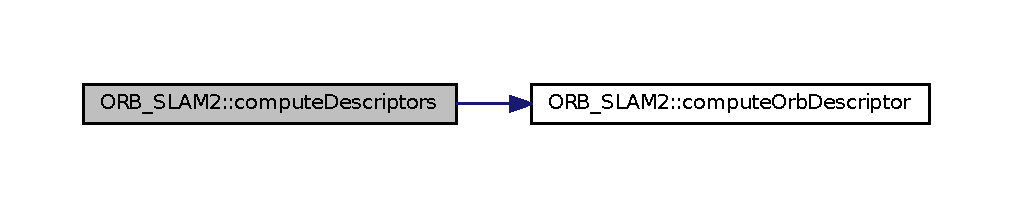
\includegraphics[width=350pt]{namespaceORB__SLAM2_ad90997cdb916a99c644c0959e08cf4df_cgraph}
\end{center}
\end{figure}


\index{O\+R\+B\+\_\+\+S\+L\+A\+M2@{O\+R\+B\+\_\+\+S\+L\+A\+M2}!compute\+Orb\+Descriptor@{compute\+Orb\+Descriptor}}
\index{compute\+Orb\+Descriptor@{compute\+Orb\+Descriptor}!O\+R\+B\+\_\+\+S\+L\+A\+M2@{O\+R\+B\+\_\+\+S\+L\+A\+M2}}
\subsubsection[{\texorpdfstring{compute\+Orb\+Descriptor(const Key\+Point \&kpt, const Mat \&img, const Point $\ast$pattern, uchar $\ast$desc)}{computeOrbDescriptor(const KeyPoint &kpt, const Mat &img, const Point *pattern, uchar *desc)}}]{\setlength{\rightskip}{0pt plus 5cm}static void O\+R\+B\+\_\+\+S\+L\+A\+M2\+::compute\+Orb\+Descriptor (
\begin{DoxyParamCaption}
\item[{const Key\+Point \&}]{kpt, }
\item[{const Mat \&}]{img, }
\item[{const Point $\ast$}]{pattern, }
\item[{uchar $\ast$}]{desc}
\end{DoxyParamCaption}
)\hspace{0.3cm}{\ttfamily [static]}}\hypertarget{namespaceORB__SLAM2_a932693f631bfe871700d02c72e14c6cd}{}\label{namespaceORB__SLAM2_a932693f631bfe871700d02c72e14c6cd}


Definition at line 108 of file O\+R\+Bextractor.\+cc.


\begin{DoxyCode}
111 \{
112     \textcolor{keywordtype}{float} angle = (float)kpt.angle*\hyperlink{namespaceORB__SLAM2_a8015b470ffeb885a0c90837a03b3210f}{factorPI};
113     \textcolor{keywordtype}{float} a = (\textcolor{keywordtype}{float})cos(angle), b = (float)sin(angle);
114 
115     \textcolor{keyword}{const} uchar* center = &img.at<uchar>(cvRound(kpt.pt.y), cvRound(kpt.pt.x));
116     \textcolor{keyword}{const} \textcolor{keywordtype}{int} step = (int)img.step;
117 
118     #define \hyperlink{ORBextractor_8cc_a35931865021519a9d7a2a4d2f196e684}{GET\_VALUE}(idx) \(\backslash\)
119         center[cvRound(pattern[idx].x*b + pattern[idx].y*a)*step + \(\backslash\)
120                cvRound(pattern[idx].x*a - pattern[idx].y*b)]
121 
122 
123     \textcolor{keywordflow}{for} (\textcolor{keywordtype}{int} i = 0; i < 32; ++i, pattern += 16)
124     \{
125         \textcolor{keywordtype}{int} t0, t1, val;
126         t0 = \hyperlink{ORBextractor_8cc_a35931865021519a9d7a2a4d2f196e684}{GET\_VALUE}(0); t1 = \hyperlink{ORBextractor_8cc_a35931865021519a9d7a2a4d2f196e684}{GET\_VALUE}(1);
127         val = t0 < t1;
128         t0 = \hyperlink{ORBextractor_8cc_a35931865021519a9d7a2a4d2f196e684}{GET\_VALUE}(2); t1 = \hyperlink{ORBextractor_8cc_a35931865021519a9d7a2a4d2f196e684}{GET\_VALUE}(3);
129         val |= (t0 < t1) << 1;
130         t0 = \hyperlink{ORBextractor_8cc_a35931865021519a9d7a2a4d2f196e684}{GET\_VALUE}(4); t1 = \hyperlink{ORBextractor_8cc_a35931865021519a9d7a2a4d2f196e684}{GET\_VALUE}(5);
131         val |= (t0 < t1) << 2;
132         t0 = \hyperlink{ORBextractor_8cc_a35931865021519a9d7a2a4d2f196e684}{GET\_VALUE}(6); t1 = \hyperlink{ORBextractor_8cc_a35931865021519a9d7a2a4d2f196e684}{GET\_VALUE}(7);
133         val |= (t0 < t1) << 3;
134         t0 = \hyperlink{ORBextractor_8cc_a35931865021519a9d7a2a4d2f196e684}{GET\_VALUE}(8); t1 = \hyperlink{ORBextractor_8cc_a35931865021519a9d7a2a4d2f196e684}{GET\_VALUE}(9);
135         val |= (t0 < t1) << 4;
136         t0 = \hyperlink{ORBextractor_8cc_a35931865021519a9d7a2a4d2f196e684}{GET\_VALUE}(10); t1 = \hyperlink{ORBextractor_8cc_a35931865021519a9d7a2a4d2f196e684}{GET\_VALUE}(11);
137         val |= (t0 < t1) << 5;
138         t0 = \hyperlink{ORBextractor_8cc_a35931865021519a9d7a2a4d2f196e684}{GET\_VALUE}(12); t1 = \hyperlink{ORBextractor_8cc_a35931865021519a9d7a2a4d2f196e684}{GET\_VALUE}(13);
139         val |= (t0 < t1) << 6;
140         t0 = \hyperlink{ORBextractor_8cc_a35931865021519a9d7a2a4d2f196e684}{GET\_VALUE}(14); t1 = \hyperlink{ORBextractor_8cc_a35931865021519a9d7a2a4d2f196e684}{GET\_VALUE}(15);
141         val |= (t0 < t1) << 7;
142 
143         desc[i] = (uchar)val;
144     \}
145 
146 \textcolor{preprocessor}{    #undef GET\_VALUE}
147 \}
\end{DoxyCode}


Here is the caller graph for this function\+:\nopagebreak
\begin{figure}[H]
\begin{center}
\leavevmode
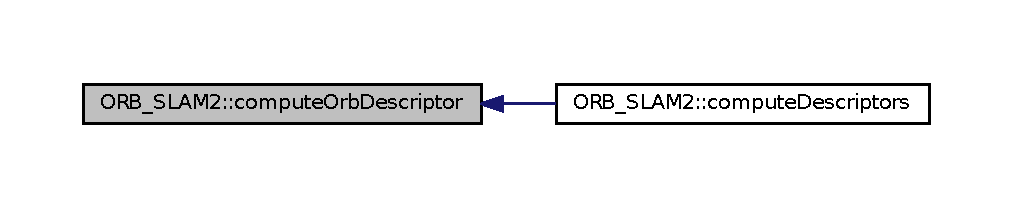
\includegraphics[width=350pt]{namespaceORB__SLAM2_a932693f631bfe871700d02c72e14c6cd_icgraph}
\end{center}
\end{figure}


\index{O\+R\+B\+\_\+\+S\+L\+A\+M2@{O\+R\+B\+\_\+\+S\+L\+A\+M2}!compute\+Orientation@{compute\+Orientation}}
\index{compute\+Orientation@{compute\+Orientation}!O\+R\+B\+\_\+\+S\+L\+A\+M2@{O\+R\+B\+\_\+\+S\+L\+A\+M2}}
\subsubsection[{\texorpdfstring{compute\+Orientation(const Mat \&image, vector$<$ Key\+Point $>$ \&keypoints, const vector$<$ int $>$ \&umax)}{computeOrientation(const Mat &image, vector< KeyPoint > &keypoints, const vector< int > &umax)}}]{\setlength{\rightskip}{0pt plus 5cm}static void O\+R\+B\+\_\+\+S\+L\+A\+M2\+::compute\+Orientation (
\begin{DoxyParamCaption}
\item[{const Mat \&}]{image, }
\item[{vector$<$ Key\+Point $>$ \&}]{keypoints, }
\item[{const vector$<$ int $>$ \&}]{umax}
\end{DoxyParamCaption}
)\hspace{0.3cm}{\ttfamily [static]}}\hypertarget{namespaceORB__SLAM2_a40adb6b621d7c2dd9d2961ba88e445c8}{}\label{namespaceORB__SLAM2_a40adb6b621d7c2dd9d2961ba88e445c8}


Definition at line 472 of file O\+R\+Bextractor.\+cc.


\begin{DoxyCode}
473 \{
474     \textcolor{keywordflow}{for} (vector<KeyPoint>::iterator keypoint = keypoints.begin(),
475          keypointEnd = keypoints.end(); keypoint != keypointEnd; ++keypoint)
476     \{
477         keypoint->angle = \hyperlink{namespaceORB__SLAM2_ac570dbdaae2d483745515b5022fd6820}{IC\_Angle}(image, keypoint->pt, umax);
478     \}
479 \}
\end{DoxyCode}


Here is the call graph for this function\+:\nopagebreak
\begin{figure}[H]
\begin{center}
\leavevmode
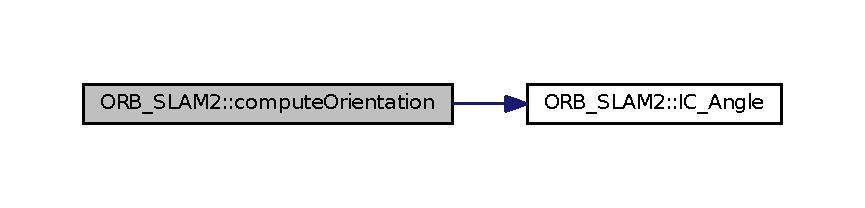
\includegraphics[width=350pt]{namespaceORB__SLAM2_a40adb6b621d7c2dd9d2961ba88e445c8_cgraph}
\end{center}
\end{figure}


\index{O\+R\+B\+\_\+\+S\+L\+A\+M2@{O\+R\+B\+\_\+\+S\+L\+A\+M2}!I\+C\+\_\+\+Angle@{I\+C\+\_\+\+Angle}}
\index{I\+C\+\_\+\+Angle@{I\+C\+\_\+\+Angle}!O\+R\+B\+\_\+\+S\+L\+A\+M2@{O\+R\+B\+\_\+\+S\+L\+A\+M2}}
\subsubsection[{\texorpdfstring{I\+C\+\_\+\+Angle(const Mat \&image, Point2f pt, const vector$<$ int $>$ \&u\+\_\+max)}{IC_Angle(const Mat &image, Point2f pt, const vector< int > &u_max)}}]{\setlength{\rightskip}{0pt plus 5cm}static float O\+R\+B\+\_\+\+S\+L\+A\+M2\+::\+I\+C\+\_\+\+Angle (
\begin{DoxyParamCaption}
\item[{const Mat \&}]{image, }
\item[{Point2f}]{pt, }
\item[{const vector$<$ int $>$ \&}]{u\+\_\+max}
\end{DoxyParamCaption}
)\hspace{0.3cm}{\ttfamily [static]}}\hypertarget{namespaceORB__SLAM2_ac570dbdaae2d483745515b5022fd6820}{}\label{namespaceORB__SLAM2_ac570dbdaae2d483745515b5022fd6820}


Definition at line 77 of file O\+R\+Bextractor.\+cc.


\begin{DoxyCode}
78 \{
79     \textcolor{keywordtype}{int} m\_01 = 0, m\_10 = 0;
80 
81     \textcolor{keyword}{const} uchar* center = &image.at<uchar> (cvRound(pt.y), cvRound(pt.x));
82 
83     \textcolor{comment}{// Treat the center line differently, v=0}
84     \textcolor{keywordflow}{for} (\textcolor{keywordtype}{int} u = -\hyperlink{namespaceORB__SLAM2_aa09849ae679bf2392b097abd710d8d7f}{HALF\_PATCH\_SIZE}; u <= \hyperlink{namespaceORB__SLAM2_aa09849ae679bf2392b097abd710d8d7f}{HALF\_PATCH\_SIZE}; ++u)
85         m\_10 += u * center[u];
86 
87     \textcolor{comment}{// Go line by line in the circuI853lar patch}
88     \textcolor{keywordtype}{int} step = (int)image.step1();
89     \textcolor{keywordflow}{for} (\textcolor{keywordtype}{int} v = 1; v <= \hyperlink{namespaceORB__SLAM2_aa09849ae679bf2392b097abd710d8d7f}{HALF\_PATCH\_SIZE}; ++v)
90     \{
91         \textcolor{comment}{// Proceed over the two lines}
92         \textcolor{keywordtype}{int} v\_sum = 0;
93         \textcolor{keywordtype}{int} d = u\_max[v];
94         \textcolor{keywordflow}{for} (\textcolor{keywordtype}{int} u = -d; u <= d; ++u)
95         \{
96             \textcolor{keywordtype}{int} val\_plus = center[u + v*step], val\_minus = center[u - v*step];
97             v\_sum += (val\_plus - val\_minus);
98             m\_10 += u * (val\_plus + val\_minus);
99         \}
100         m\_01 += v * v\_sum;
101     \}
102 
103     \textcolor{keywordflow}{return} fastAtan2((\textcolor{keywordtype}{float})m\_01, (\textcolor{keywordtype}{float})m\_10);
104 \}
\end{DoxyCode}


Here is the caller graph for this function\+:\nopagebreak
\begin{figure}[H]
\begin{center}
\leavevmode
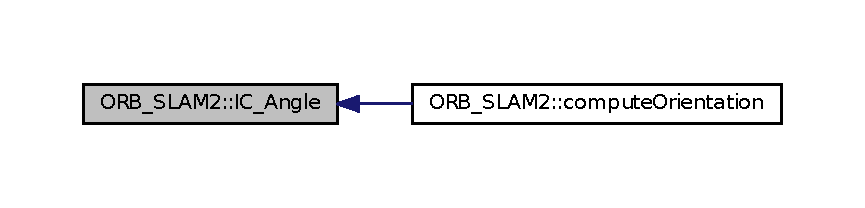
\includegraphics[width=350pt]{namespaceORB__SLAM2_ac570dbdaae2d483745515b5022fd6820_icgraph}
\end{center}
\end{figure}




\subsection{Variable Documentation}
\index{O\+R\+B\+\_\+\+S\+L\+A\+M2@{O\+R\+B\+\_\+\+S\+L\+A\+M2}!bit\+\_\+pattern\+\_\+31\+\_\+@{bit\+\_\+pattern\+\_\+31\+\_\+}}
\index{bit\+\_\+pattern\+\_\+31\+\_\+@{bit\+\_\+pattern\+\_\+31\+\_\+}!O\+R\+B\+\_\+\+S\+L\+A\+M2@{O\+R\+B\+\_\+\+S\+L\+A\+M2}}
\subsubsection[{\texorpdfstring{bit\+\_\+pattern\+\_\+31\+\_\+}{bit_pattern_31_}}]{\setlength{\rightskip}{0pt plus 5cm}int O\+R\+B\+\_\+\+S\+L\+A\+M2\+::bit\+\_\+pattern\+\_\+31\+\_\+\mbox{[}256 $\ast$4\mbox{]}\hspace{0.3cm}{\ttfamily [static]}}\hypertarget{namespaceORB__SLAM2_a8dd21ee063eca2b0bc3f5e76ceba0492}{}\label{namespaceORB__SLAM2_a8dd21ee063eca2b0bc3f5e76ceba0492}


Definition at line 150 of file O\+R\+Bextractor.\+cc.

\index{O\+R\+B\+\_\+\+S\+L\+A\+M2@{O\+R\+B\+\_\+\+S\+L\+A\+M2}!E\+D\+G\+E\+\_\+\+T\+H\+R\+E\+S\+H\+O\+LD@{E\+D\+G\+E\+\_\+\+T\+H\+R\+E\+S\+H\+O\+LD}}
\index{E\+D\+G\+E\+\_\+\+T\+H\+R\+E\+S\+H\+O\+LD@{E\+D\+G\+E\+\_\+\+T\+H\+R\+E\+S\+H\+O\+LD}!O\+R\+B\+\_\+\+S\+L\+A\+M2@{O\+R\+B\+\_\+\+S\+L\+A\+M2}}
\subsubsection[{\texorpdfstring{E\+D\+G\+E\+\_\+\+T\+H\+R\+E\+S\+H\+O\+LD}{EDGE_THRESHOLD}}]{\setlength{\rightskip}{0pt plus 5cm}const int O\+R\+B\+\_\+\+S\+L\+A\+M2\+::\+E\+D\+G\+E\+\_\+\+T\+H\+R\+E\+S\+H\+O\+LD = 19}\hypertarget{namespaceORB__SLAM2_aec00f1ad4dea35755e3af4404282cd3b}{}\label{namespaceORB__SLAM2_aec00f1ad4dea35755e3af4404282cd3b}


Definition at line 74 of file O\+R\+Bextractor.\+cc.

\index{O\+R\+B\+\_\+\+S\+L\+A\+M2@{O\+R\+B\+\_\+\+S\+L\+A\+M2}!factor\+PI@{factor\+PI}}
\index{factor\+PI@{factor\+PI}!O\+R\+B\+\_\+\+S\+L\+A\+M2@{O\+R\+B\+\_\+\+S\+L\+A\+M2}}
\subsubsection[{\texorpdfstring{factor\+PI}{factorPI}}]{\setlength{\rightskip}{0pt plus 5cm}const float O\+R\+B\+\_\+\+S\+L\+A\+M2\+::factor\+PI = (float)(C\+V\+\_\+\+PI/180.f)}\hypertarget{namespaceORB__SLAM2_a8015b470ffeb885a0c90837a03b3210f}{}\label{namespaceORB__SLAM2_a8015b470ffeb885a0c90837a03b3210f}


Definition at line 107 of file O\+R\+Bextractor.\+cc.

\index{O\+R\+B\+\_\+\+S\+L\+A\+M2@{O\+R\+B\+\_\+\+S\+L\+A\+M2}!H\+A\+L\+F\+\_\+\+P\+A\+T\+C\+H\+\_\+\+S\+I\+ZE@{H\+A\+L\+F\+\_\+\+P\+A\+T\+C\+H\+\_\+\+S\+I\+ZE}}
\index{H\+A\+L\+F\+\_\+\+P\+A\+T\+C\+H\+\_\+\+S\+I\+ZE@{H\+A\+L\+F\+\_\+\+P\+A\+T\+C\+H\+\_\+\+S\+I\+ZE}!O\+R\+B\+\_\+\+S\+L\+A\+M2@{O\+R\+B\+\_\+\+S\+L\+A\+M2}}
\subsubsection[{\texorpdfstring{H\+A\+L\+F\+\_\+\+P\+A\+T\+C\+H\+\_\+\+S\+I\+ZE}{HALF_PATCH_SIZE}}]{\setlength{\rightskip}{0pt plus 5cm}const int O\+R\+B\+\_\+\+S\+L\+A\+M2\+::\+H\+A\+L\+F\+\_\+\+P\+A\+T\+C\+H\+\_\+\+S\+I\+ZE = 15}\hypertarget{namespaceORB__SLAM2_aa09849ae679bf2392b097abd710d8d7f}{}\label{namespaceORB__SLAM2_aa09849ae679bf2392b097abd710d8d7f}


Definition at line 73 of file O\+R\+Bextractor.\+cc.

\index{O\+R\+B\+\_\+\+S\+L\+A\+M2@{O\+R\+B\+\_\+\+S\+L\+A\+M2}!P\+A\+T\+C\+H\+\_\+\+S\+I\+ZE@{P\+A\+T\+C\+H\+\_\+\+S\+I\+ZE}}
\index{P\+A\+T\+C\+H\+\_\+\+S\+I\+ZE@{P\+A\+T\+C\+H\+\_\+\+S\+I\+ZE}!O\+R\+B\+\_\+\+S\+L\+A\+M2@{O\+R\+B\+\_\+\+S\+L\+A\+M2}}
\subsubsection[{\texorpdfstring{P\+A\+T\+C\+H\+\_\+\+S\+I\+ZE}{PATCH_SIZE}}]{\setlength{\rightskip}{0pt plus 5cm}const int O\+R\+B\+\_\+\+S\+L\+A\+M2\+::\+P\+A\+T\+C\+H\+\_\+\+S\+I\+ZE = 31}\hypertarget{namespaceORB__SLAM2_a557e5c298c5f7164667f083494c2197a}{}\label{namespaceORB__SLAM2_a557e5c298c5f7164667f083494c2197a}


Definition at line 72 of file O\+R\+Bextractor.\+cc.


\chapter{Class Documentation}
\hypertarget{classMatAllocator}{}\section{Mat\+Allocator Class Reference}
\label{classMatAllocator}\index{Mat\+Allocator@{Mat\+Allocator}}


Inheritance diagram for Mat\+Allocator\+:\nopagebreak
\begin{figure}[H]
\begin{center}
\leavevmode
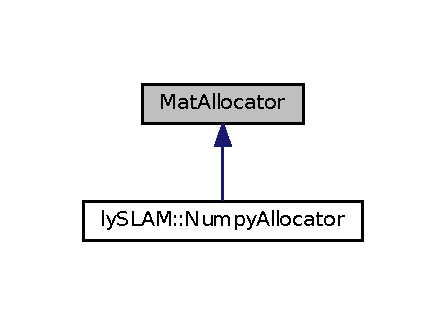
\includegraphics[width=214pt]{classMatAllocator__inherit__graph}
\end{center}
\end{figure}


The documentation for this class was generated from the following file\+:\begin{DoxyCompactItemize}
\item 
\hyperlink{Conversion_8cc}{Conversion.\+cc}\end{DoxyCompactItemize}

\hypertarget{classlySLAM_1_1NumpyAllocator}{}\section{ly\+S\+L\+AM\+:\+:Numpy\+Allocator Class Reference}
\label{classlySLAM_1_1NumpyAllocator}\index{ly\+S\+L\+A\+M\+::\+Numpy\+Allocator@{ly\+S\+L\+A\+M\+::\+Numpy\+Allocator}}


Inheritance diagram for ly\+S\+L\+AM\+:\+:Numpy\+Allocator\+:\nopagebreak
\begin{figure}[H]
\begin{center}
\leavevmode
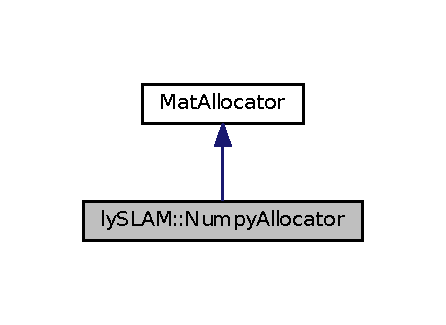
\includegraphics[width=214pt]{classlySLAM_1_1NumpyAllocator__inherit__graph}
\end{center}
\end{figure}


Collaboration diagram for ly\+S\+L\+AM\+:\+:Numpy\+Allocator\+:\nopagebreak
\begin{figure}[H]
\begin{center}
\leavevmode
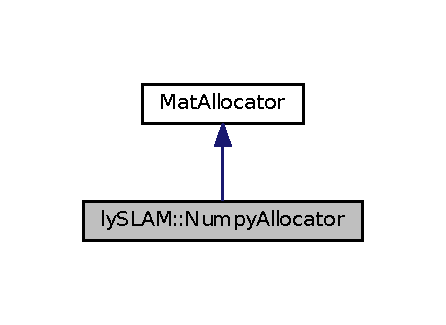
\includegraphics[width=214pt]{classlySLAM_1_1NumpyAllocator__coll__graph}
\end{center}
\end{figure}
\subsection*{Public Member Functions}
\begin{DoxyCompactItemize}
\item 
\hyperlink{classlySLAM_1_1NumpyAllocator_af955f14c0c1758b47841ba26f01d2799}{Numpy\+Allocator} ()
\item 
\hyperlink{classlySLAM_1_1NumpyAllocator_a444dd279208d905a277bbd7027dc274b}{$\sim$\+Numpy\+Allocator} ()
\item 
void \hyperlink{classlySLAM_1_1NumpyAllocator_a871b654d21f5bebe682fefeeaa24d02f}{allocate} (int dims, const int $\ast$sizes, int type, int $\ast$\&refcount, uchar $\ast$\&datastart, uchar $\ast$\&data, size\+\_\+t $\ast$step)
\item 
void \hyperlink{classlySLAM_1_1NumpyAllocator_a7568a09a23ce22ace5425f5bdd327c75}{deallocate} (int $\ast$refcount, uchar $\ast$, uchar $\ast$)
\end{DoxyCompactItemize}


\subsection{Detailed Description}


Definition at line 74 of file Conversion.\+cc.



\subsection{Constructor \& Destructor Documentation}
\index{ly\+S\+L\+A\+M\+::\+Numpy\+Allocator@{ly\+S\+L\+A\+M\+::\+Numpy\+Allocator}!Numpy\+Allocator@{Numpy\+Allocator}}
\index{Numpy\+Allocator@{Numpy\+Allocator}!ly\+S\+L\+A\+M\+::\+Numpy\+Allocator@{ly\+S\+L\+A\+M\+::\+Numpy\+Allocator}}
\subsubsection[{\texorpdfstring{Numpy\+Allocator()}{NumpyAllocator()}}]{\setlength{\rightskip}{0pt plus 5cm}ly\+S\+L\+A\+M\+::\+Numpy\+Allocator\+::\+Numpy\+Allocator (
\begin{DoxyParamCaption}
{}
\end{DoxyParamCaption}
)\hspace{0.3cm}{\ttfamily [inline]}}\hypertarget{classlySLAM_1_1NumpyAllocator_af955f14c0c1758b47841ba26f01d2799}{}\label{classlySLAM_1_1NumpyAllocator_af955f14c0c1758b47841ba26f01d2799}


Definition at line 77 of file Conversion.\+cc.


\begin{DoxyCode}
77 \{\}
\end{DoxyCode}
\index{ly\+S\+L\+A\+M\+::\+Numpy\+Allocator@{ly\+S\+L\+A\+M\+::\+Numpy\+Allocator}!````~Numpy\+Allocator@{$\sim$\+Numpy\+Allocator}}
\index{````~Numpy\+Allocator@{$\sim$\+Numpy\+Allocator}!ly\+S\+L\+A\+M\+::\+Numpy\+Allocator@{ly\+S\+L\+A\+M\+::\+Numpy\+Allocator}}
\subsubsection[{\texorpdfstring{$\sim$\+Numpy\+Allocator()}{~NumpyAllocator()}}]{\setlength{\rightskip}{0pt plus 5cm}ly\+S\+L\+A\+M\+::\+Numpy\+Allocator\+::$\sim$\+Numpy\+Allocator (
\begin{DoxyParamCaption}
{}
\end{DoxyParamCaption}
)\hspace{0.3cm}{\ttfamily [inline]}}\hypertarget{classlySLAM_1_1NumpyAllocator_a444dd279208d905a277bbd7027dc274b}{}\label{classlySLAM_1_1NumpyAllocator_a444dd279208d905a277bbd7027dc274b}


Definition at line 78 of file Conversion.\+cc.


\begin{DoxyCode}
78 \{\}
\end{DoxyCode}


\subsection{Member Function Documentation}
\index{ly\+S\+L\+A\+M\+::\+Numpy\+Allocator@{ly\+S\+L\+A\+M\+::\+Numpy\+Allocator}!allocate@{allocate}}
\index{allocate@{allocate}!ly\+S\+L\+A\+M\+::\+Numpy\+Allocator@{ly\+S\+L\+A\+M\+::\+Numpy\+Allocator}}
\subsubsection[{\texorpdfstring{allocate(int dims, const int $\ast$sizes, int type, int $\ast$\&refcount, uchar $\ast$\&datastart, uchar $\ast$\&data, size\+\_\+t $\ast$step)}{allocate(int dims, const int *sizes, int type, int *&refcount, uchar *&datastart, uchar *&data, size_t *step)}}]{\setlength{\rightskip}{0pt plus 5cm}void ly\+S\+L\+A\+M\+::\+Numpy\+Allocator\+::allocate (
\begin{DoxyParamCaption}
\item[{int}]{dims, }
\item[{const int $\ast$}]{sizes, }
\item[{int}]{type, }
\item[{int $\ast$\&}]{refcount, }
\item[{uchar $\ast$\&}]{datastart, }
\item[{uchar $\ast$\&}]{data, }
\item[{size\+\_\+t $\ast$}]{step}
\end{DoxyParamCaption}
)\hspace{0.3cm}{\ttfamily [inline]}}\hypertarget{classlySLAM_1_1NumpyAllocator_a871b654d21f5bebe682fefeeaa24d02f}{}\label{classlySLAM_1_1NumpyAllocator_a871b654d21f5bebe682fefeeaa24d02f}


Definition at line 80 of file Conversion.\+cc.


\begin{DoxyCode}
82     \{
83 
84         \textcolor{comment}{//PyEnsureGIL gil;}
85 
86         \textcolor{keywordtype}{int} depth = CV\_MAT\_DEPTH(type);
87         \textcolor{keywordtype}{int} cn = CV\_MAT\_CN(type);
88 
89         \textcolor{keyword}{const} \textcolor{keywordtype}{int} f = (int)(\textcolor{keyword}{sizeof}(\textcolor{keywordtype}{size\_t})/8);
90         \textcolor{keywordtype}{int} typenum = depth == CV\_8U ? NPY\_UBYTE : depth == CV\_8S ? NPY\_BYTE :
91                                                                     depth == CV\_16U ? NPY\_USHORT : depth ==
       CV\_16S ? NPY\_SHORT :
92                                                                                                            
                depth == CV\_32S ? NPY\_INT : depth == CV\_32F ? NPY\_FLOAT :
93                                                                                                            
                                                              depth == CV\_64F ? NPY\_DOUBLE : f*NPY\_ULONGLONG + (f^
      1)*NPY\_UINT;
94         \textcolor{keywordtype}{int} i;
95 
96         npy\_intp \_sizes[CV\_MAX\_DIM+1];
97         \textcolor{keywordflow}{for}( i = 0; i < dims; i++ )
98         \{
99             \_sizes[i] = sizes[i];
100         \}
101 
102         \textcolor{keywordflow}{if}( cn > 1 )
103         \{
104             \_sizes[dims++] = cn;
105         \}
106         PyObject* o = PyArray\_SimpleNew(dims, \_sizes, typenum);
107         \textcolor{keywordflow}{if}(!o)
108         \{
109 
110             CV\_Error\_(CV\_StsError, (\textcolor{stringliteral}{"The numpy array of typenum=%d, ndims=%d can not be created"}, typenum, 
      dims));
111         \}
112         refcount = refcountFromPyObject(o);
113 
114         npy\_intp* \_strides = PyArray\_STRIDES(o);
115         \textcolor{keywordflow}{for}( i = 0; i < dims - (cn > 1); i++ )
116             step[i] = (\textcolor{keywordtype}{size\_t})\_strides[i];
117 
118         datastart = data = (uchar*) PyArray\_DATA(o);
119 
120     \}
\end{DoxyCode}
\index{ly\+S\+L\+A\+M\+::\+Numpy\+Allocator@{ly\+S\+L\+A\+M\+::\+Numpy\+Allocator}!deallocate@{deallocate}}
\index{deallocate@{deallocate}!ly\+S\+L\+A\+M\+::\+Numpy\+Allocator@{ly\+S\+L\+A\+M\+::\+Numpy\+Allocator}}
\subsubsection[{\texorpdfstring{deallocate(int $\ast$refcount, uchar $\ast$, uchar $\ast$)}{deallocate(int *refcount, uchar *, uchar *)}}]{\setlength{\rightskip}{0pt plus 5cm}void ly\+S\+L\+A\+M\+::\+Numpy\+Allocator\+::deallocate (
\begin{DoxyParamCaption}
\item[{int $\ast$}]{refcount, }
\item[{uchar $\ast$}]{, }
\item[{uchar $\ast$}]{}
\end{DoxyParamCaption}
)\hspace{0.3cm}{\ttfamily [inline]}}\hypertarget{classlySLAM_1_1NumpyAllocator_a7568a09a23ce22ace5425f5bdd327c75}{}\label{classlySLAM_1_1NumpyAllocator_a7568a09a23ce22ace5425f5bdd327c75}


Definition at line 122 of file Conversion.\+cc.


\begin{DoxyCode}
123     \{
124         \textcolor{comment}{//PyEnsureGIL gil;}
125         \textcolor{keywordflow}{if}( !refcount )
126             \textcolor{keywordflow}{return};
127         PyObject* o = pyObjectFromRefcount(refcount);
128         Py\_INCREF(o);
129         Py\_DECREF(o);
130     \}
\end{DoxyCode}


The documentation for this class was generated from the following file\+:\begin{DoxyCompactItemize}
\item 
\hyperlink{Conversion_8cc}{Conversion.\+cc}\end{DoxyCompactItemize}

\hypertarget{classlySLAM_1_1PyAllowThreads}{}\section{ly\+S\+L\+AM\+:\+:Py\+Allow\+Threads Class Reference}
\label{classlySLAM_1_1PyAllowThreads}\index{ly\+S\+L\+A\+M\+::\+Py\+Allow\+Threads@{ly\+S\+L\+A\+M\+::\+Py\+Allow\+Threads}}


Collaboration diagram for ly\+S\+L\+AM\+:\+:Py\+Allow\+Threads\+:\nopagebreak
\begin{figure}[H]
\begin{center}
\leavevmode
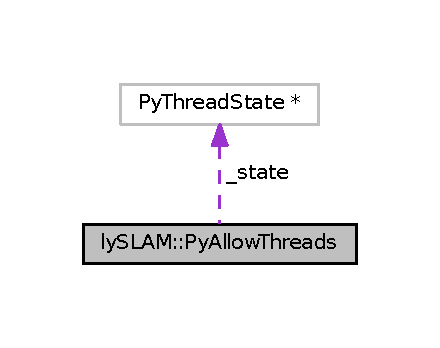
\includegraphics[width=211pt]{classlySLAM_1_1PyAllowThreads__coll__graph}
\end{center}
\end{figure}
\subsection*{Public Member Functions}
\begin{DoxyCompactItemize}
\item 
\hyperlink{classlySLAM_1_1PyAllowThreads_ab8568add3eada88f40c00d1b5b30b0ad}{Py\+Allow\+Threads} ()
\item 
\hyperlink{classlySLAM_1_1PyAllowThreads_adcdfe6fcc17c17aa09079691e055bd9d}{$\sim$\+Py\+Allow\+Threads} ()
\end{DoxyCompactItemize}
\subsection*{Private Attributes}
\begin{DoxyCompactItemize}
\item 
Py\+Thread\+State $\ast$ \hyperlink{classlySLAM_1_1PyAllowThreads_ac8076cd04c356e648d9ae5e28cd0d4aa}{\+\_\+state}
\end{DoxyCompactItemize}


\subsection{Detailed Description}


Definition at line 34 of file Conversion.\+cc.



\subsection{Constructor \& Destructor Documentation}
\index{ly\+S\+L\+A\+M\+::\+Py\+Allow\+Threads@{ly\+S\+L\+A\+M\+::\+Py\+Allow\+Threads}!Py\+Allow\+Threads@{Py\+Allow\+Threads}}
\index{Py\+Allow\+Threads@{Py\+Allow\+Threads}!ly\+S\+L\+A\+M\+::\+Py\+Allow\+Threads@{ly\+S\+L\+A\+M\+::\+Py\+Allow\+Threads}}
\subsubsection[{\texorpdfstring{Py\+Allow\+Threads()}{PyAllowThreads()}}]{\setlength{\rightskip}{0pt plus 5cm}ly\+S\+L\+A\+M\+::\+Py\+Allow\+Threads\+::\+Py\+Allow\+Threads (
\begin{DoxyParamCaption}
{}
\end{DoxyParamCaption}
)\hspace{0.3cm}{\ttfamily [inline]}}\hypertarget{classlySLAM_1_1PyAllowThreads_ab8568add3eada88f40c00d1b5b30b0ad}{}\label{classlySLAM_1_1PyAllowThreads_ab8568add3eada88f40c00d1b5b30b0ad}


Definition at line 37 of file Conversion.\+cc.


\begin{DoxyCode}
37 : \hyperlink{classlySLAM_1_1PyAllowThreads_ac8076cd04c356e648d9ae5e28cd0d4aa}{\_state}(PyEval\_SaveThread()) \{\}
\end{DoxyCode}
\index{ly\+S\+L\+A\+M\+::\+Py\+Allow\+Threads@{ly\+S\+L\+A\+M\+::\+Py\+Allow\+Threads}!````~Py\+Allow\+Threads@{$\sim$\+Py\+Allow\+Threads}}
\index{````~Py\+Allow\+Threads@{$\sim$\+Py\+Allow\+Threads}!ly\+S\+L\+A\+M\+::\+Py\+Allow\+Threads@{ly\+S\+L\+A\+M\+::\+Py\+Allow\+Threads}}
\subsubsection[{\texorpdfstring{$\sim$\+Py\+Allow\+Threads()}{~PyAllowThreads()}}]{\setlength{\rightskip}{0pt plus 5cm}ly\+S\+L\+A\+M\+::\+Py\+Allow\+Threads\+::$\sim$\+Py\+Allow\+Threads (
\begin{DoxyParamCaption}
{}
\end{DoxyParamCaption}
)\hspace{0.3cm}{\ttfamily [inline]}}\hypertarget{classlySLAM_1_1PyAllowThreads_adcdfe6fcc17c17aa09079691e055bd9d}{}\label{classlySLAM_1_1PyAllowThreads_adcdfe6fcc17c17aa09079691e055bd9d}


Definition at line 38 of file Conversion.\+cc.


\begin{DoxyCode}
39     \{
40         PyEval\_RestoreThread(\hyperlink{classlySLAM_1_1PyAllowThreads_ac8076cd04c356e648d9ae5e28cd0d4aa}{\_state});
41     \}
\end{DoxyCode}


\subsection{Member Data Documentation}
\index{ly\+S\+L\+A\+M\+::\+Py\+Allow\+Threads@{ly\+S\+L\+A\+M\+::\+Py\+Allow\+Threads}!\+\_\+state@{\+\_\+state}}
\index{\+\_\+state@{\+\_\+state}!ly\+S\+L\+A\+M\+::\+Py\+Allow\+Threads@{ly\+S\+L\+A\+M\+::\+Py\+Allow\+Threads}}
\subsubsection[{\texorpdfstring{\+\_\+state}{_state}}]{\setlength{\rightskip}{0pt plus 5cm}Py\+Thread\+State$\ast$ ly\+S\+L\+A\+M\+::\+Py\+Allow\+Threads\+::\+\_\+state\hspace{0.3cm}{\ttfamily [private]}}\hypertarget{classlySLAM_1_1PyAllowThreads_ac8076cd04c356e648d9ae5e28cd0d4aa}{}\label{classlySLAM_1_1PyAllowThreads_ac8076cd04c356e648d9ae5e28cd0d4aa}


Definition at line 43 of file Conversion.\+cc.



The documentation for this class was generated from the following file\+:\begin{DoxyCompactItemize}
\item 
\hyperlink{Conversion_8cc}{Conversion.\+cc}\end{DoxyCompactItemize}

\hypertarget{classlySLAM_1_1PyEnsureGIL}{}\section{ly\+S\+L\+AM\+:\+:Py\+Ensure\+G\+IL Class Reference}
\label{classlySLAM_1_1PyEnsureGIL}\index{ly\+S\+L\+A\+M\+::\+Py\+Ensure\+G\+IL@{ly\+S\+L\+A\+M\+::\+Py\+Ensure\+G\+IL}}


Collaboration diagram for ly\+S\+L\+AM\+:\+:Py\+Ensure\+G\+IL\+:\nopagebreak
\begin{figure}[H]
\begin{center}
\leavevmode
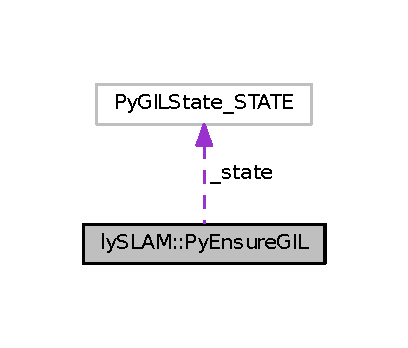
\includegraphics[width=196pt]{classlySLAM_1_1PyEnsureGIL__coll__graph}
\end{center}
\end{figure}
\subsection*{Public Member Functions}
\begin{DoxyCompactItemize}
\item 
\hyperlink{classlySLAM_1_1PyEnsureGIL_a1b7f914c64f03eaf053e2854925d620a}{Py\+Ensure\+G\+IL} ()
\item 
\hyperlink{classlySLAM_1_1PyEnsureGIL_a39bb4f6f02bbd598d89819ddd2b90529}{$\sim$\+Py\+Ensure\+G\+IL} ()
\end{DoxyCompactItemize}
\subsection*{Private Attributes}
\begin{DoxyCompactItemize}
\item 
Py\+G\+I\+L\+State\+\_\+\+S\+T\+A\+TE \hyperlink{classlySLAM_1_1PyEnsureGIL_ade2080afcd63201ae95bb0eb5bfd3696}{\+\_\+state}
\end{DoxyCompactItemize}


\subsection{Detailed Description}


Definition at line 46 of file Conversion.\+cc.



\subsection{Constructor \& Destructor Documentation}
\index{ly\+S\+L\+A\+M\+::\+Py\+Ensure\+G\+IL@{ly\+S\+L\+A\+M\+::\+Py\+Ensure\+G\+IL}!Py\+Ensure\+G\+IL@{Py\+Ensure\+G\+IL}}
\index{Py\+Ensure\+G\+IL@{Py\+Ensure\+G\+IL}!ly\+S\+L\+A\+M\+::\+Py\+Ensure\+G\+IL@{ly\+S\+L\+A\+M\+::\+Py\+Ensure\+G\+IL}}
\subsubsection[{\texorpdfstring{Py\+Ensure\+G\+I\+L()}{PyEnsureGIL()}}]{\setlength{\rightskip}{0pt plus 5cm}ly\+S\+L\+A\+M\+::\+Py\+Ensure\+G\+I\+L\+::\+Py\+Ensure\+G\+IL (
\begin{DoxyParamCaption}
{}
\end{DoxyParamCaption}
)\hspace{0.3cm}{\ttfamily [inline]}}\hypertarget{classlySLAM_1_1PyEnsureGIL_a1b7f914c64f03eaf053e2854925d620a}{}\label{classlySLAM_1_1PyEnsureGIL_a1b7f914c64f03eaf053e2854925d620a}


Definition at line 49 of file Conversion.\+cc.


\begin{DoxyCode}
49 : \hyperlink{classlySLAM_1_1PyEnsureGIL_ade2080afcd63201ae95bb0eb5bfd3696}{\_state}(PyGILState\_Ensure()) \{\}
\end{DoxyCode}
\index{ly\+S\+L\+A\+M\+::\+Py\+Ensure\+G\+IL@{ly\+S\+L\+A\+M\+::\+Py\+Ensure\+G\+IL}!````~Py\+Ensure\+G\+IL@{$\sim$\+Py\+Ensure\+G\+IL}}
\index{````~Py\+Ensure\+G\+IL@{$\sim$\+Py\+Ensure\+G\+IL}!ly\+S\+L\+A\+M\+::\+Py\+Ensure\+G\+IL@{ly\+S\+L\+A\+M\+::\+Py\+Ensure\+G\+IL}}
\subsubsection[{\texorpdfstring{$\sim$\+Py\+Ensure\+G\+I\+L()}{~PyEnsureGIL()}}]{\setlength{\rightskip}{0pt plus 5cm}ly\+S\+L\+A\+M\+::\+Py\+Ensure\+G\+I\+L\+::$\sim$\+Py\+Ensure\+G\+IL (
\begin{DoxyParamCaption}
{}
\end{DoxyParamCaption}
)\hspace{0.3cm}{\ttfamily [inline]}}\hypertarget{classlySLAM_1_1PyEnsureGIL_a39bb4f6f02bbd598d89819ddd2b90529}{}\label{classlySLAM_1_1PyEnsureGIL_a39bb4f6f02bbd598d89819ddd2b90529}


Definition at line 50 of file Conversion.\+cc.


\begin{DoxyCode}
51     \{
52         std::cout << \textcolor{stringliteral}{"releasing"}<< std::endl;
53         PyGILState\_Release(\hyperlink{classlySLAM_1_1PyEnsureGIL_ade2080afcd63201ae95bb0eb5bfd3696}{\_state});
54     \}
\end{DoxyCode}


\subsection{Member Data Documentation}
\index{ly\+S\+L\+A\+M\+::\+Py\+Ensure\+G\+IL@{ly\+S\+L\+A\+M\+::\+Py\+Ensure\+G\+IL}!\+\_\+state@{\+\_\+state}}
\index{\+\_\+state@{\+\_\+state}!ly\+S\+L\+A\+M\+::\+Py\+Ensure\+G\+IL@{ly\+S\+L\+A\+M\+::\+Py\+Ensure\+G\+IL}}
\subsubsection[{\texorpdfstring{\+\_\+state}{_state}}]{\setlength{\rightskip}{0pt plus 5cm}Py\+G\+I\+L\+State\+\_\+\+S\+T\+A\+TE ly\+S\+L\+A\+M\+::\+Py\+Ensure\+G\+I\+L\+::\+\_\+state\hspace{0.3cm}{\ttfamily [private]}}\hypertarget{classlySLAM_1_1PyEnsureGIL_ade2080afcd63201ae95bb0eb5bfd3696}{}\label{classlySLAM_1_1PyEnsureGIL_ade2080afcd63201ae95bb0eb5bfd3696}


Definition at line 56 of file Conversion.\+cc.



The documentation for this class was generated from the following file\+:\begin{DoxyCompactItemize}
\item 
\hyperlink{Conversion_8cc}{Conversion.\+cc}\end{DoxyCompactItemize}

\chapter{File Documentation}
\hypertarget{Conversion_8cc}{}\section{Conversion.\+cc File Reference}
\label{Conversion_8cc}\index{Conversion.\+cc@{Conversion.\+cc}}
{\ttfamily \#include $<$iostream$>$}\\*
{\ttfamily \#include \char`\"{}Conversion.\+h\char`\"{}}\\*
Include dependency graph for Conversion.\+cc\+:\nopagebreak
\begin{figure}[H]
\begin{center}
\leavevmode
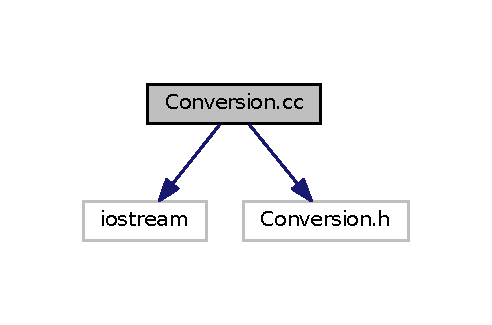
\includegraphics[width=236pt]{Conversion_8cc__incl}
\end{center}
\end{figure}
\subsection*{Classes}
\begin{DoxyCompactItemize}
\item 
class \hyperlink{classlySLAM_1_1PyAllowThreads}{ly\+S\+L\+A\+M\+::\+Py\+Allow\+Threads}
\item 
class \hyperlink{classlySLAM_1_1PyEnsureGIL}{ly\+S\+L\+A\+M\+::\+Py\+Ensure\+G\+IL}
\item 
class \hyperlink{classlySLAM_1_1NumpyAllocator}{ly\+S\+L\+A\+M\+::\+Numpy\+Allocator}
\end{DoxyCompactItemize}
\subsection*{Namespaces}
\begin{DoxyCompactItemize}
\item 
 \hyperlink{namespacelySLAM}{ly\+S\+L\+AM}
\end{DoxyCompactItemize}
\subsection*{Functions}
\begin{DoxyCompactItemize}
\item 
static void \hyperlink{namespacelySLAM_a00b314520d011d12b2bd631293ea02a8}{ly\+S\+L\+A\+M\+::init} ()
\item 
static int \hyperlink{namespacelySLAM_a7b41c0e11cbb97ca1485abd44d51e799}{ly\+S\+L\+A\+M\+::failmsg} (const char $\ast$fmt,...)
\item 
static Py\+Object $\ast$ \hyperlink{namespacelySLAM_a4c4e113b266fb98524f7c06154fe33e1}{ly\+S\+L\+A\+M\+::failmsgp} (const char $\ast$fmt,...)
\end{DoxyCompactItemize}
\subsection*{Variables}
\begin{DoxyCompactItemize}
\item 
Numpy\+Allocator \hyperlink{namespacelySLAM_a487059d3e4df5c492791c26d6316a9f2}{ly\+S\+L\+A\+M\+::g\+\_\+numpy\+Allocator}
\end{DoxyCompactItemize}

\hypertarget{Converter_8cc}{}\section{Converter.\+cc File Reference}
\label{Converter_8cc}\index{Converter.\+cc@{Converter.\+cc}}
{\ttfamily \#include \char`\"{}Converter.\+h\char`\"{}}\\*
Include dependency graph for Converter.\+cc\+:\nopagebreak
\begin{figure}[H]
\begin{center}
\leavevmode
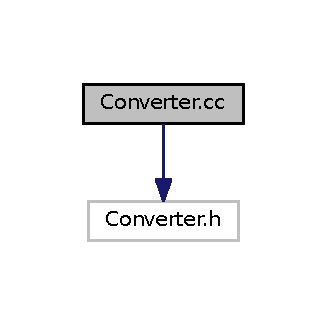
\includegraphics[width=157pt]{Converter_8cc__incl}
\end{center}
\end{figure}
\subsection*{Namespaces}
\begin{DoxyCompactItemize}
\item 
 \hyperlink{namespaceORB__SLAM2}{O\+R\+B\+\_\+\+S\+L\+A\+M2}
\end{DoxyCompactItemize}

\hypertarget{Frame_8cc}{}\section{Frame.\+cc File Reference}
\label{Frame_8cc}\index{Frame.\+cc@{Frame.\+cc}}
{\ttfamily \#include \char`\"{}Frame.\+h\char`\"{}}\\*
{\ttfamily \#include \char`\"{}Converter.\+h\char`\"{}}\\*
{\ttfamily \#include \char`\"{}O\+R\+Bmatcher.\+h\char`\"{}}\\*
{\ttfamily \#include $<$thread$>$}\\*
{\ttfamily \#include \char`\"{}Semantic.\+h\char`\"{}}\\*
Include dependency graph for Frame.\+cc\+:\nopagebreak
\begin{figure}[H]
\begin{center}
\leavevmode
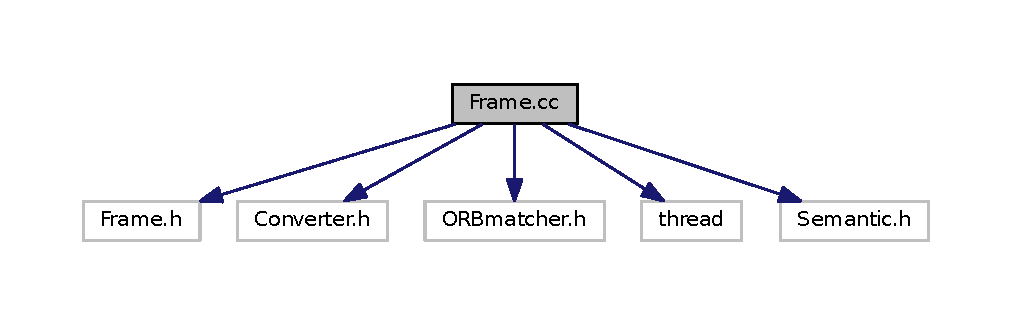
\includegraphics[width=350pt]{Frame_8cc__incl}
\end{center}
\end{figure}
\subsection*{Namespaces}
\begin{DoxyCompactItemize}
\item 
 \hyperlink{namespaceORB__SLAM2}{O\+R\+B\+\_\+\+S\+L\+A\+M2}
\end{DoxyCompactItemize}

\hypertarget{FrameDrawer_8cc}{}\section{Frame\+Drawer.\+cc File Reference}
\label{FrameDrawer_8cc}\index{Frame\+Drawer.\+cc@{Frame\+Drawer.\+cc}}
{\ttfamily \#include \char`\"{}Frame\+Drawer.\+h\char`\"{}}\\*
{\ttfamily \#include \char`\"{}Tracking.\+h\char`\"{}}\\*
{\ttfamily \#include $<$opencv2/core/core.\+hpp$>$}\\*
{\ttfamily \#include $<$opencv2/highgui/highgui.\+hpp$>$}\\*
{\ttfamily \#include $<$mutex$>$}\\*
Include dependency graph for Frame\+Drawer.\+cc\+:\nopagebreak
\begin{figure}[H]
\begin{center}
\leavevmode
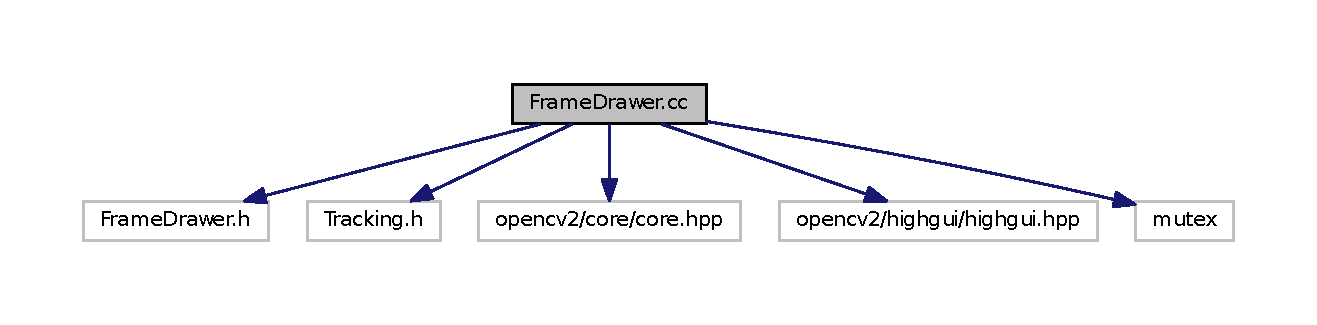
\includegraphics[width=350pt]{FrameDrawer_8cc__incl}
\end{center}
\end{figure}
\subsection*{Namespaces}
\begin{DoxyCompactItemize}
\item 
 \hyperlink{namespaceORB__SLAM2}{O\+R\+B\+\_\+\+S\+L\+A\+M2}
\end{DoxyCompactItemize}

\hypertarget{Geometry_8cc}{}\section{Geometry.\+cc File Reference}
\label{Geometry_8cc}\index{Geometry.\+cc@{Geometry.\+cc}}
{\ttfamily \#include \char`\"{}Geometry.\+h\char`\"{}}\\*
{\ttfamily \#include $<$algorithm$>$}\\*
{\ttfamily \#include \char`\"{}Frame.\+h\char`\"{}}\\*
{\ttfamily \#include \char`\"{}Tracking.\+h\char`\"{}}\\*
Include dependency graph for Geometry.\+cc\+:\nopagebreak
\begin{figure}[H]
\begin{center}
\leavevmode
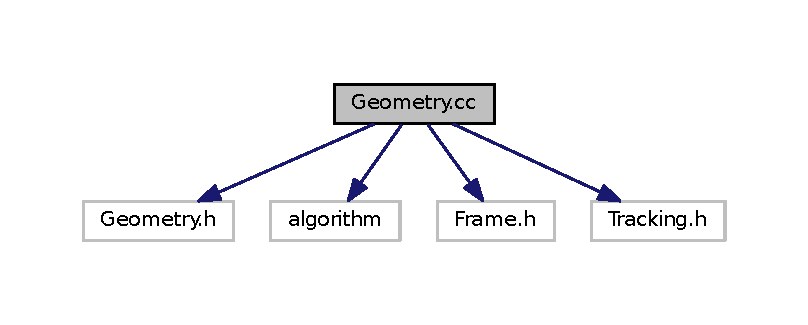
\includegraphics[width=350pt]{Geometry_8cc__incl}
\end{center}
\end{figure}
\subsection*{Namespaces}
\begin{DoxyCompactItemize}
\item 
 \hyperlink{namespacelySLAM}{ly\+S\+L\+AM}
\end{DoxyCompactItemize}
\subsection*{Functions}
\begin{DoxyCompactItemize}
\item 
float \hyperlink{namespacelySLAM_a432cf91e1b1dee06c5d9a35cc1b5529a}{ly\+S\+L\+A\+M\+::\+Area} (float x1, float x2, float y1, float y2)
\end{DoxyCompactItemize}

\hypertarget{Initializer_8cc}{}\section{Initializer.\+cc File Reference}
\label{Initializer_8cc}\index{Initializer.\+cc@{Initializer.\+cc}}
{\ttfamily \#include \char`\"{}Initializer.\+h\char`\"{}}\\*
{\ttfamily \#include \char`\"{}Thirdparty/\+D\+Bo\+W2/\+D\+Utils/\+Random.\+h\char`\"{}}\\*
{\ttfamily \#include \char`\"{}Optimizer.\+h\char`\"{}}\\*
{\ttfamily \#include \char`\"{}O\+R\+Bmatcher.\+h\char`\"{}}\\*
{\ttfamily \#include $<$thread$>$}\\*
Include dependency graph for Initializer.\+cc\+:\nopagebreak
\begin{figure}[H]
\begin{center}
\leavevmode
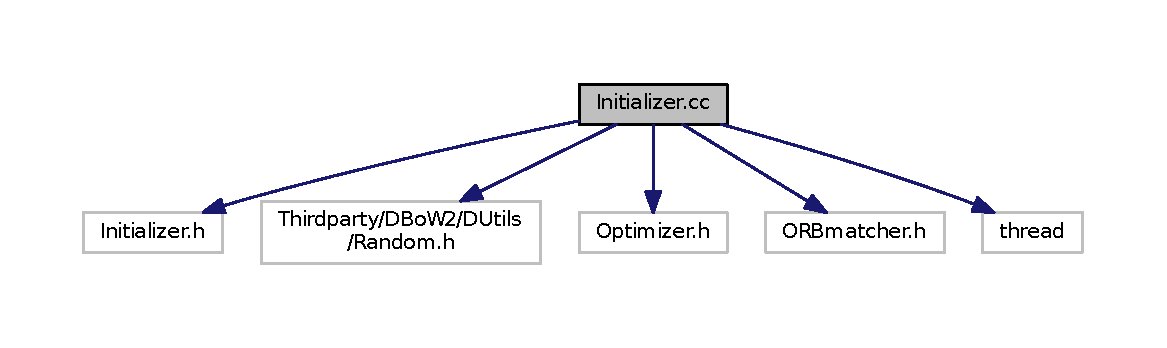
\includegraphics[width=350pt]{Initializer_8cc__incl}
\end{center}
\end{figure}
\subsection*{Namespaces}
\begin{DoxyCompactItemize}
\item 
 \hyperlink{namespaceORB__SLAM2}{O\+R\+B\+\_\+\+S\+L\+A\+M2}
\end{DoxyCompactItemize}

\hypertarget{KeyFrame_8cc}{}\section{Key\+Frame.\+cc File Reference}
\label{KeyFrame_8cc}\index{Key\+Frame.\+cc@{Key\+Frame.\+cc}}
{\ttfamily \#include \char`\"{}Key\+Frame.\+h\char`\"{}}\\*
{\ttfamily \#include \char`\"{}Converter.\+h\char`\"{}}\\*
{\ttfamily \#include \char`\"{}O\+R\+Bmatcher.\+h\char`\"{}}\\*
{\ttfamily \#include $<$mutex$>$}\\*
{\ttfamily \#include \char`\"{}Semantic.\+h\char`\"{}}\\*
Include dependency graph for Key\+Frame.\+cc\+:\nopagebreak
\begin{figure}[H]
\begin{center}
\leavevmode
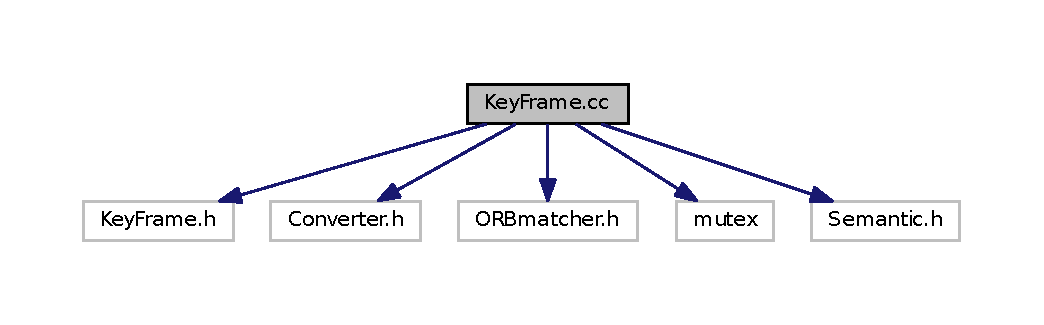
\includegraphics[width=350pt]{KeyFrame_8cc__incl}
\end{center}
\end{figure}
\subsection*{Namespaces}
\begin{DoxyCompactItemize}
\item 
 \hyperlink{namespaceORB__SLAM2}{O\+R\+B\+\_\+\+S\+L\+A\+M2}
\end{DoxyCompactItemize}

\hypertarget{KeyFrameDatabase_8cc}{}\section{Key\+Frame\+Database.\+cc File Reference}
\label{KeyFrameDatabase_8cc}\index{Key\+Frame\+Database.\+cc@{Key\+Frame\+Database.\+cc}}
{\ttfamily \#include \char`\"{}Key\+Frame\+Database.\+h\char`\"{}}\\*
{\ttfamily \#include \char`\"{}Key\+Frame.\+h\char`\"{}}\\*
{\ttfamily \#include \char`\"{}Thirdparty/\+D\+Bo\+W2/\+D\+Bo\+W2/\+Bow\+Vector.\+h\char`\"{}}\\*
{\ttfamily \#include $<$mutex$>$}\\*
Include dependency graph for Key\+Frame\+Database.\+cc\+:\nopagebreak
\begin{figure}[H]
\begin{center}
\leavevmode
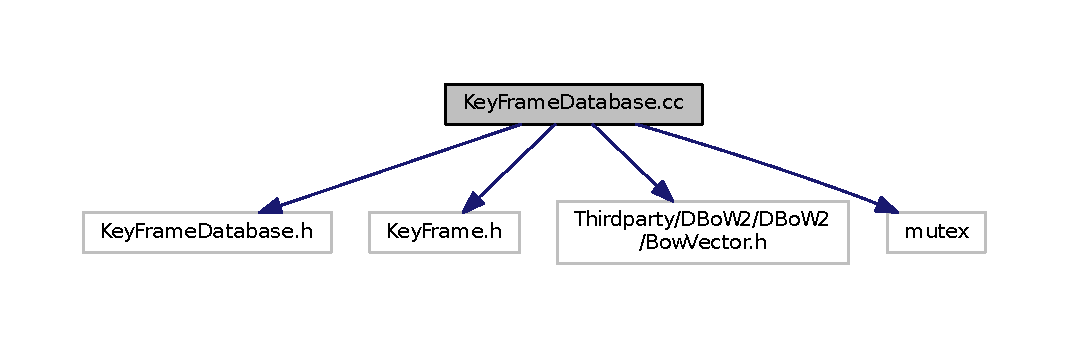
\includegraphics[width=350pt]{KeyFrameDatabase_8cc__incl}
\end{center}
\end{figure}
\subsection*{Namespaces}
\begin{DoxyCompactItemize}
\item 
 \hyperlink{namespaceORB__SLAM2}{O\+R\+B\+\_\+\+S\+L\+A\+M2}
\end{DoxyCompactItemize}

\hypertarget{LocalMapping_8cc}{}\section{Local\+Mapping.\+cc File Reference}
\label{LocalMapping_8cc}\index{Local\+Mapping.\+cc@{Local\+Mapping.\+cc}}
{\ttfamily \#include \char`\"{}Local\+Mapping.\+h\char`\"{}}\\*
{\ttfamily \#include \char`\"{}Loop\+Closing.\+h\char`\"{}}\\*
{\ttfamily \#include \char`\"{}O\+R\+Bmatcher.\+h\char`\"{}}\\*
{\ttfamily \#include \char`\"{}Optimizer.\+h\char`\"{}}\\*
{\ttfamily \#include $<$unistd.\+h$>$}\\*
{\ttfamily \#include $<$mutex$>$}\\*
Include dependency graph for Local\+Mapping.\+cc\+:\nopagebreak
\begin{figure}[H]
\begin{center}
\leavevmode
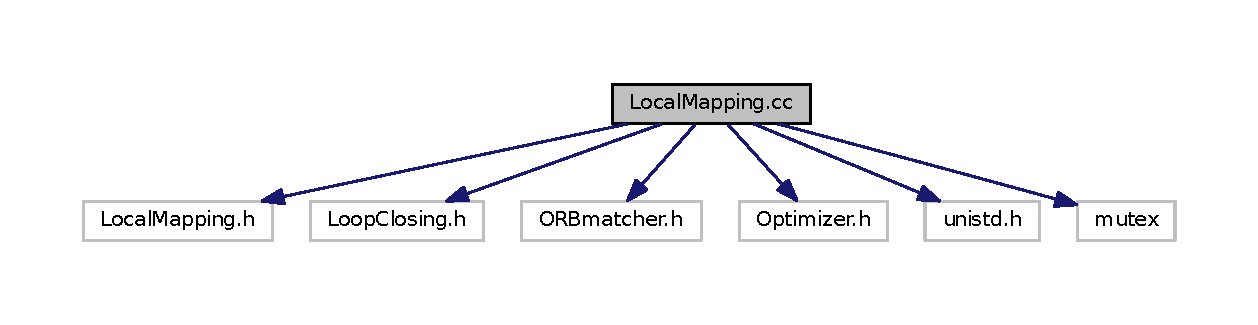
\includegraphics[width=350pt]{LocalMapping_8cc__incl}
\end{center}
\end{figure}
\subsection*{Namespaces}
\begin{DoxyCompactItemize}
\item 
 \hyperlink{namespaceORB__SLAM2}{O\+R\+B\+\_\+\+S\+L\+A\+M2}
\end{DoxyCompactItemize}

\hypertarget{LoopClosing_8cc}{}\section{Loop\+Closing.\+cc File Reference}
\label{LoopClosing_8cc}\index{Loop\+Closing.\+cc@{Loop\+Closing.\+cc}}
{\ttfamily \#include \char`\"{}Loop\+Closing.\+h\char`\"{}}\\*
{\ttfamily \#include \char`\"{}Sim3\+Solver.\+h\char`\"{}}\\*
{\ttfamily \#include \char`\"{}Converter.\+h\char`\"{}}\\*
{\ttfamily \#include \char`\"{}Optimizer.\+h\char`\"{}}\\*
{\ttfamily \#include \char`\"{}O\+R\+Bmatcher.\+h\char`\"{}}\\*
{\ttfamily \#include $<$unistd.\+h$>$}\\*
{\ttfamily \#include $<$mutex$>$}\\*
{\ttfamily \#include $<$thread$>$}\\*
Include dependency graph for Loop\+Closing.\+cc\+:\nopagebreak
\begin{figure}[H]
\begin{center}
\leavevmode
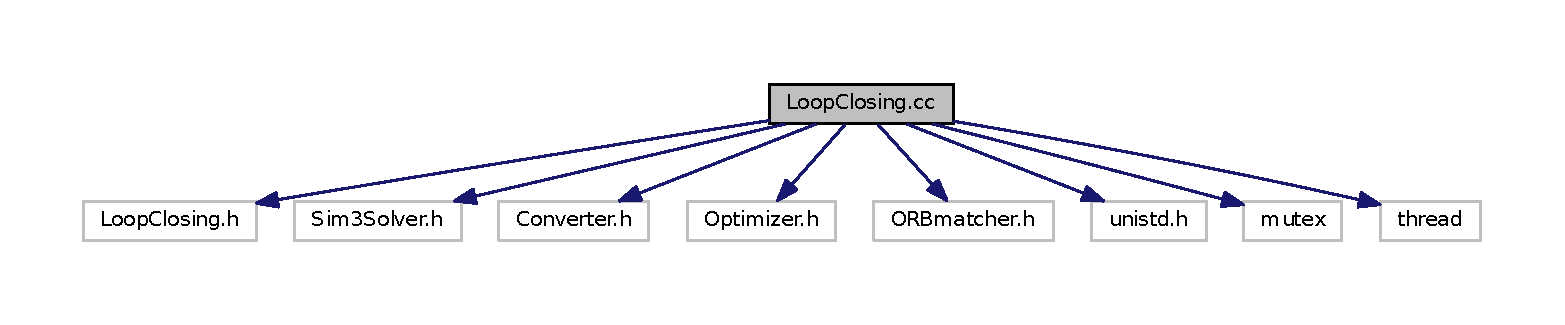
\includegraphics[width=350pt]{LoopClosing_8cc__incl}
\end{center}
\end{figure}
\subsection*{Namespaces}
\begin{DoxyCompactItemize}
\item 
 \hyperlink{namespaceORB__SLAM2}{O\+R\+B\+\_\+\+S\+L\+A\+M2}
\end{DoxyCompactItemize}

\hypertarget{Map_8cc}{}\section{Map.\+cc File Reference}
\label{Map_8cc}\index{Map.\+cc@{Map.\+cc}}
{\ttfamily \#include \char`\"{}Map.\+h\char`\"{}}\\*
{\ttfamily \#include $<$mutex$>$}\\*
Include dependency graph for Map.\+cc\+:\nopagebreak
\begin{figure}[H]
\begin{center}
\leavevmode
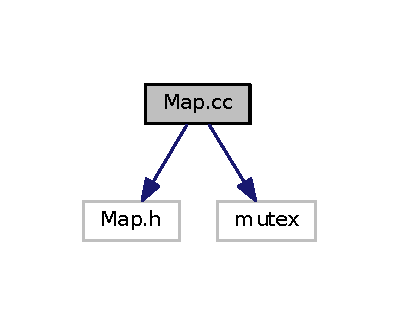
\includegraphics[width=192pt]{Map_8cc__incl}
\end{center}
\end{figure}
\subsection*{Namespaces}
\begin{DoxyCompactItemize}
\item 
 \hyperlink{namespaceORB__SLAM2}{O\+R\+B\+\_\+\+S\+L\+A\+M2}
\end{DoxyCompactItemize}

\hypertarget{MapDrawer_8cc}{}\section{Map\+Drawer.\+cc File Reference}
\label{MapDrawer_8cc}\index{Map\+Drawer.\+cc@{Map\+Drawer.\+cc}}
{\ttfamily \#include \char`\"{}Map\+Drawer.\+h\char`\"{}}\\*
{\ttfamily \#include \char`\"{}Map\+Point.\+h\char`\"{}}\\*
{\ttfamily \#include \char`\"{}Key\+Frame.\+h\char`\"{}}\\*
{\ttfamily \#include $<$pangolin/pangolin.\+h$>$}\\*
{\ttfamily \#include $<$mutex$>$}\\*
Include dependency graph for Map\+Drawer.\+cc\+:\nopagebreak
\begin{figure}[H]
\begin{center}
\leavevmode
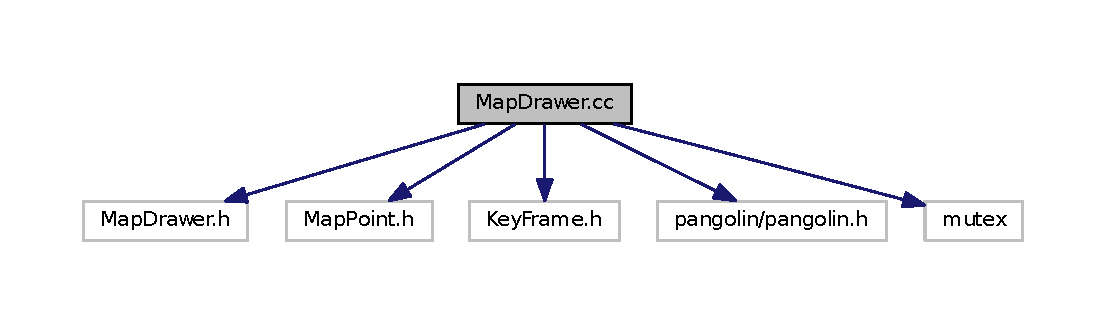
\includegraphics[width=350pt]{MapDrawer_8cc__incl}
\end{center}
\end{figure}
\subsection*{Namespaces}
\begin{DoxyCompactItemize}
\item 
 \hyperlink{namespaceORB__SLAM2}{O\+R\+B\+\_\+\+S\+L\+A\+M2}
\end{DoxyCompactItemize}

\hypertarget{MapPoint_8cc}{}\section{Map\+Point.\+cc File Reference}
\label{MapPoint_8cc}\index{Map\+Point.\+cc@{Map\+Point.\+cc}}
{\ttfamily \#include \char`\"{}Map\+Point.\+h\char`\"{}}\\*
{\ttfamily \#include \char`\"{}O\+R\+Bmatcher.\+h\char`\"{}}\\*
{\ttfamily \#include $<$mutex$>$}\\*
Include dependency graph for Map\+Point.\+cc\+:\nopagebreak
\begin{figure}[H]
\begin{center}
\leavevmode
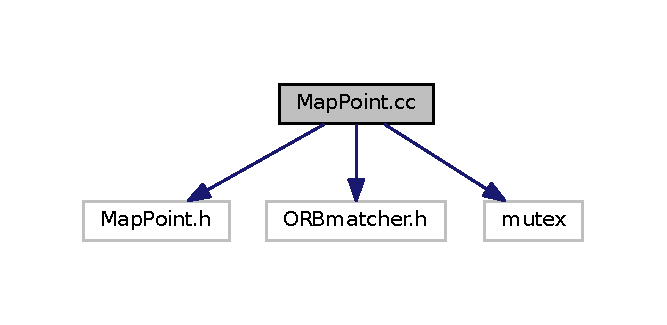
\includegraphics[width=320pt]{MapPoint_8cc__incl}
\end{center}
\end{figure}
\subsection*{Namespaces}
\begin{DoxyCompactItemize}
\item 
 \hyperlink{namespaceORB__SLAM2}{O\+R\+B\+\_\+\+S\+L\+A\+M2}
\end{DoxyCompactItemize}

\hypertarget{MaskNet_8cc}{}\section{Mask\+Net.\+cc File Reference}
\label{MaskNet_8cc}\index{Mask\+Net.\+cc@{Mask\+Net.\+cc}}
{\ttfamily \#include \char`\"{}Common.\+h\char`\"{}}\\*
{\ttfamily \#include \char`\"{}Mask\+Net.\+h\char`\"{}}\\*
{\ttfamily \#include $<$iostream$>$}\\*
{\ttfamily \#include $<$fstream$>$}\\*
{\ttfamily \#include $<$iomanip$>$}\\*
{\ttfamily \#include $<$dirent.\+h$>$}\\*
{\ttfamily \#include $<$errno.\+h$>$}\\*
Include dependency graph for Mask\+Net.\+cc\+:\nopagebreak
\begin{figure}[H]
\begin{center}
\leavevmode
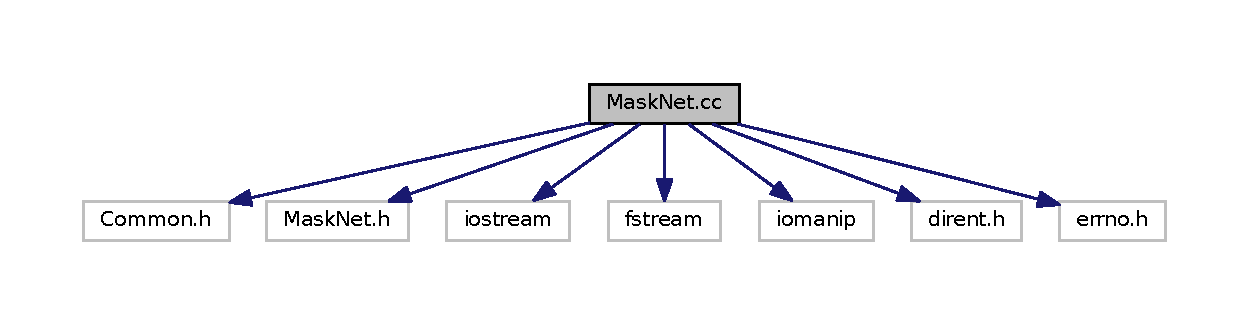
\includegraphics[width=350pt]{MaskNet_8cc__incl}
\end{center}
\end{figure}
\subsection*{Namespaces}
\begin{DoxyCompactItemize}
\item 
 \hyperlink{namespacelySLAM}{ly\+S\+L\+AM}
\end{DoxyCompactItemize}
\subsection*{Macros}
\begin{DoxyCompactItemize}
\item 
\#define \hyperlink{MaskNet_8cc_a8e5d338049896ac5a96c5b617e3e543a}{U\+\_\+\+S\+E\+G\+St}(a)
\end{DoxyCompactItemize}
\subsection*{Functions}
\begin{DoxyCompactItemize}
\item 
void \hyperlink{namespacelySLAM_a83245374bbce9e47c4878b5613fb98db}{ly\+S\+L\+A\+M\+::tic\+\_\+initsv} ()
\item 
void \hyperlink{namespacelySLAM_adb77bc91beb203170ca5a301968f9f76}{ly\+S\+L\+A\+M\+::toc\+\_\+finalsv} (double \&time)
\item 
void \hyperlink{namespacelySLAM_af18d8f81de160c1de261c5465c29523e}{ly\+S\+L\+A\+M\+::ticsv} ()
\item 
void \hyperlink{namespacelySLAM_a56e5af1fe2c6086f5597b0e44465ffc3}{ly\+S\+L\+A\+M\+::tocsv} ()
\end{DoxyCompactItemize}
\subsection*{Variables}
\begin{DoxyCompactItemize}
\item 
struct timeval \hyperlink{namespacelySLAM_a823e029c6b9b89870dc987acb8e9c032}{ly\+S\+L\+A\+M\+::tvsv}
\item 
double \hyperlink{namespacelySLAM_ab1de636cddc68247bbed233099d643f9}{ly\+S\+L\+A\+M\+::t1sv}
\item 
double \hyperlink{namespacelySLAM_a6b5e057f8ce421fbc6d49a07ef7e3273}{ly\+S\+L\+A\+M\+::t2sv}
\item 
double \hyperlink{namespacelySLAM_aee2bcc68912513a06dfc54c894ae3efc}{ly\+S\+L\+A\+M\+::t0sv}
\item 
double \hyperlink{namespacelySLAM_a76440f183e00c79997868ddfe1dae982}{ly\+S\+L\+A\+M\+::t3sv}
\end{DoxyCompactItemize}


\subsection{Macro Definition Documentation}
\index{Mask\+Net.\+cc@{Mask\+Net.\+cc}!U\+\_\+\+S\+E\+G\+St@{U\+\_\+\+S\+E\+G\+St}}
\index{U\+\_\+\+S\+E\+G\+St@{U\+\_\+\+S\+E\+G\+St}!Mask\+Net.\+cc@{Mask\+Net.\+cc}}
\subsubsection[{\texorpdfstring{U\+\_\+\+S\+E\+G\+St}{U_SEGSt}}]{\setlength{\rightskip}{0pt plus 5cm}\#define U\+\_\+\+S\+E\+G\+St(
\begin{DoxyParamCaption}
\item[{}]{a}
\end{DoxyParamCaption}
)}\hypertarget{MaskNet_8cc_a8e5d338049896ac5a96c5b617e3e543a}{}\label{MaskNet_8cc_a8e5d338049896ac5a96c5b617e3e543a}
{\bfseries Value\+:}
\begin{DoxyCode}
gettimeofday(&\hyperlink{namespacelySLAM_a823e029c6b9b89870dc987acb8e9c032}{tvsv},0);\(\backslash\)
    a = \hyperlink{namespacelySLAM_a823e029c6b9b89870dc987acb8e9c032}{tvsv}.tv\_sec + \hyperlink{namespacelySLAM_a823e029c6b9b89870dc987acb8e9c032}{tvsv}.tv\_usec/1000000.0
\end{DoxyCode}


Definition at line 21 of file Mask\+Net.\+cc.


\hypertarget{MaskNetStereo_8cc}{}\section{Mask\+Net\+Stereo.\+cc File Reference}
\label{MaskNetStereo_8cc}\index{Mask\+Net\+Stereo.\+cc@{Mask\+Net\+Stereo.\+cc}}
{\ttfamily \#include \char`\"{}Mask\+Net.\+h\char`\"{}}\\*
{\ttfamily \#include $<$iostream$>$}\\*
{\ttfamily \#include $<$fstream$>$}\\*
{\ttfamily \#include $<$iomanip$>$}\\*
Include dependency graph for Mask\+Net\+Stereo.\+cc\+:\nopagebreak
\begin{figure}[H]
\begin{center}
\leavevmode
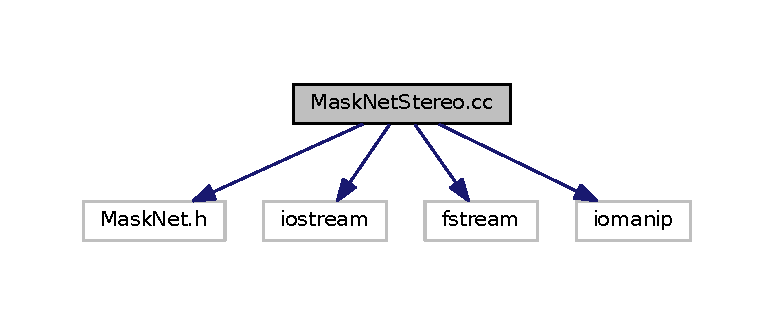
\includegraphics[width=350pt]{MaskNetStereo_8cc__incl}
\end{center}
\end{figure}
\subsection*{Namespaces}
\begin{DoxyCompactItemize}
\item 
 \hyperlink{namespacelySLAM}{ly\+S\+L\+AM}
\end{DoxyCompactItemize}

\hypertarget{Optimizer_8cc}{}\section{Optimizer.\+cc File Reference}
\label{Optimizer_8cc}\index{Optimizer.\+cc@{Optimizer.\+cc}}
{\ttfamily \#include \char`\"{}Optimizer.\+h\char`\"{}}\\*
{\ttfamily \#include \char`\"{}Thirdparty/g2o/g2o/core/block\+\_\+solver.\+h\char`\"{}}\\*
{\ttfamily \#include \char`\"{}Thirdparty/g2o/g2o/core/optimization\+\_\+algorithm\+\_\+levenberg.\+h\char`\"{}}\\*
{\ttfamily \#include \char`\"{}Thirdparty/g2o/g2o/solvers/linear\+\_\+solver\+\_\+eigen.\+h\char`\"{}}\\*
{\ttfamily \#include \char`\"{}Thirdparty/g2o/g2o/types/types\+\_\+six\+\_\+dof\+\_\+expmap.\+h\char`\"{}}\\*
{\ttfamily \#include \char`\"{}Thirdparty/g2o/g2o/core/robust\+\_\+kernel\+\_\+impl.\+h\char`\"{}}\\*
{\ttfamily \#include \char`\"{}Thirdparty/g2o/g2o/solvers/linear\+\_\+solver\+\_\+dense.\+h\char`\"{}}\\*
{\ttfamily \#include \char`\"{}Thirdparty/g2o/g2o/types/types\+\_\+seven\+\_\+dof\+\_\+expmap.\+h\char`\"{}}\\*
{\ttfamily \#include $<$Eigen/\+Std\+Vector$>$}\\*
{\ttfamily \#include \char`\"{}Converter.\+h\char`\"{}}\\*
{\ttfamily \#include $<$mutex$>$}\\*
Include dependency graph for Optimizer.\+cc\+:\nopagebreak
\begin{figure}[H]
\begin{center}
\leavevmode
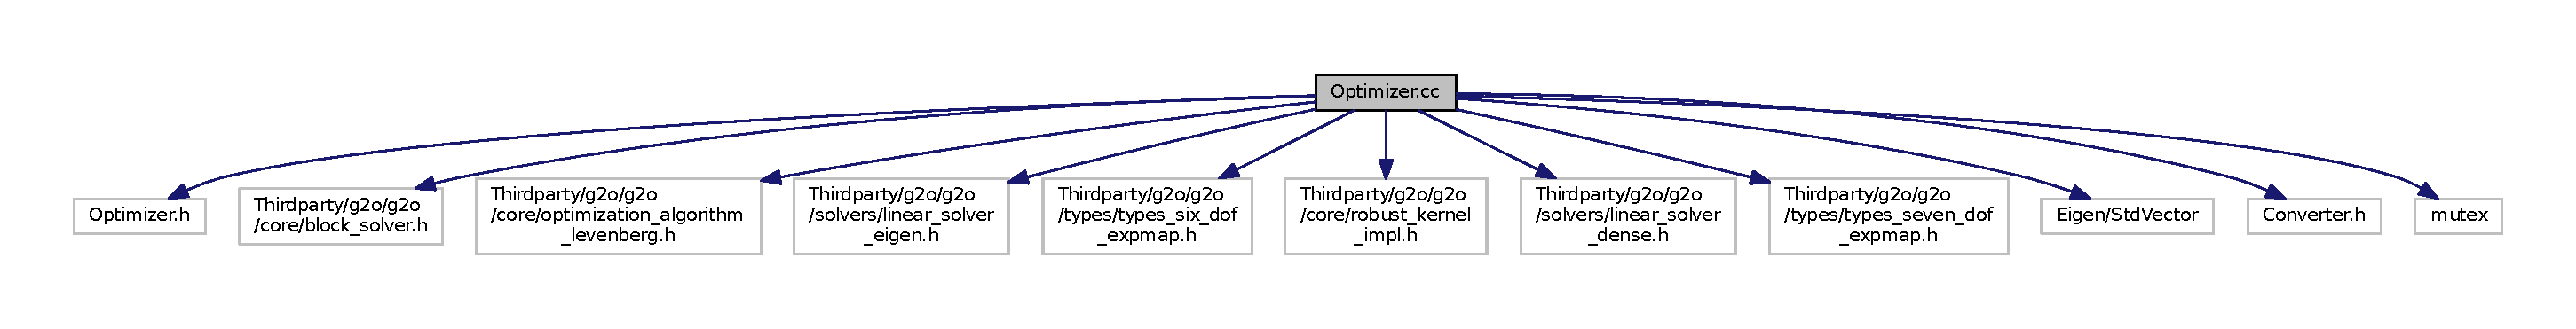
\includegraphics[width=350pt]{Optimizer_8cc__incl}
\end{center}
\end{figure}
\subsection*{Namespaces}
\begin{DoxyCompactItemize}
\item 
 \hyperlink{namespaceORB__SLAM2}{O\+R\+B\+\_\+\+S\+L\+A\+M2}
\end{DoxyCompactItemize}

\hypertarget{ORBextractor_8cc}{}\section{O\+R\+Bextractor.\+cc File Reference}
\label{ORBextractor_8cc}\index{O\+R\+Bextractor.\+cc@{O\+R\+Bextractor.\+cc}}
{\ttfamily \#include $<$opencv2/core/core.\+hpp$>$}\\*
{\ttfamily \#include $<$opencv2/highgui/highgui.\+hpp$>$}\\*
{\ttfamily \#include $<$opencv2/features2d/features2d.\+hpp$>$}\\*
{\ttfamily \#include $<$opencv2/imgproc/imgproc.\+hpp$>$}\\*
{\ttfamily \#include $<$vector$>$}\\*
{\ttfamily \#include \char`\"{}O\+R\+Bextractor.\+h\char`\"{}}\\*
Include dependency graph for O\+R\+Bextractor.\+cc\+:\nopagebreak
\begin{figure}[H]
\begin{center}
\leavevmode
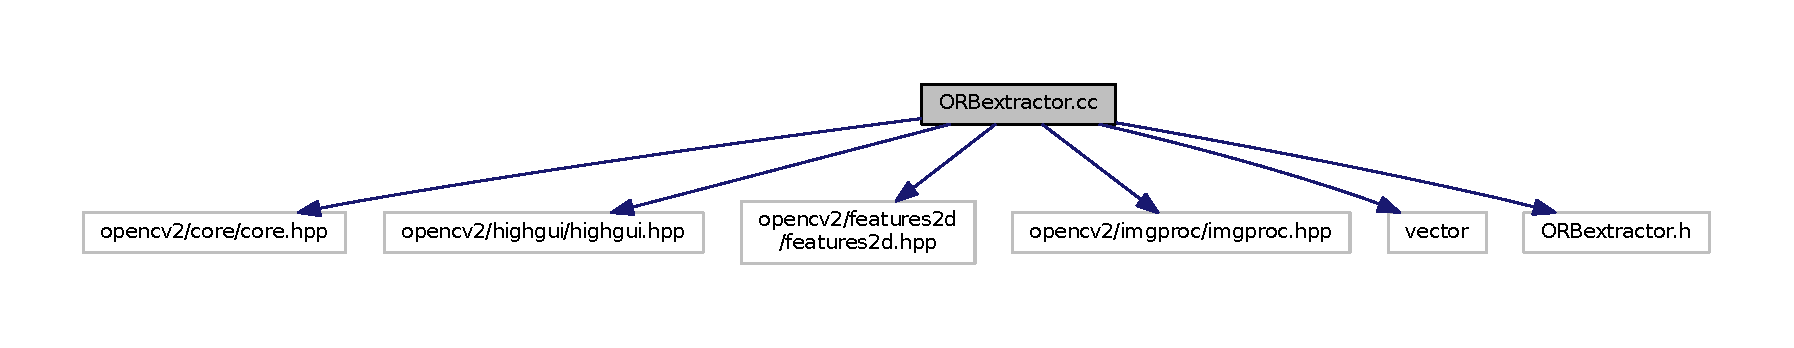
\includegraphics[width=350pt]{ORBextractor_8cc__incl}
\end{center}
\end{figure}
\subsection*{Namespaces}
\begin{DoxyCompactItemize}
\item 
 \hyperlink{namespaceORB__SLAM2}{O\+R\+B\+\_\+\+S\+L\+A\+M2}
\end{DoxyCompactItemize}
\subsection*{Macros}
\begin{DoxyCompactItemize}
\item 
\#define \hyperlink{ORBextractor_8cc_a35931865021519a9d7a2a4d2f196e684}{G\+E\+T\+\_\+\+V\+A\+L\+UE}(idx)
\end{DoxyCompactItemize}
\subsection*{Functions}
\begin{DoxyCompactItemize}
\item 
static float \hyperlink{namespaceORB__SLAM2_ac570dbdaae2d483745515b5022fd6820}{O\+R\+B\+\_\+\+S\+L\+A\+M2\+::\+I\+C\+\_\+\+Angle} (const Mat \&image, Point2f pt, const vector$<$ int $>$ \&u\+\_\+max)
\item 
static void \hyperlink{namespaceORB__SLAM2_a932693f631bfe871700d02c72e14c6cd}{O\+R\+B\+\_\+\+S\+L\+A\+M2\+::compute\+Orb\+Descriptor} (const Key\+Point \&kpt, const Mat \&img, const Point $\ast$pattern, uchar $\ast$desc)
\item 
static void \hyperlink{namespaceORB__SLAM2_a40adb6b621d7c2dd9d2961ba88e445c8}{O\+R\+B\+\_\+\+S\+L\+A\+M2\+::compute\+Orientation} (const Mat \&image, vector$<$ Key\+Point $>$ \&keypoints, const vector$<$ int $>$ \&umax)
\item 
static void \hyperlink{namespaceORB__SLAM2_ad90997cdb916a99c644c0959e08cf4df}{O\+R\+B\+\_\+\+S\+L\+A\+M2\+::compute\+Descriptors} (const Mat \&image, vector$<$ Key\+Point $>$ \&keypoints, Mat \&descriptors, const vector$<$ Point $>$ \&pattern)
\end{DoxyCompactItemize}
\subsection*{Variables}
\begin{DoxyCompactItemize}
\item 
const int \hyperlink{namespaceORB__SLAM2_a557e5c298c5f7164667f083494c2197a}{O\+R\+B\+\_\+\+S\+L\+A\+M2\+::\+P\+A\+T\+C\+H\+\_\+\+S\+I\+ZE} = 31
\item 
const int \hyperlink{namespaceORB__SLAM2_aa09849ae679bf2392b097abd710d8d7f}{O\+R\+B\+\_\+\+S\+L\+A\+M2\+::\+H\+A\+L\+F\+\_\+\+P\+A\+T\+C\+H\+\_\+\+S\+I\+ZE} = 15
\item 
const int \hyperlink{namespaceORB__SLAM2_aec00f1ad4dea35755e3af4404282cd3b}{O\+R\+B\+\_\+\+S\+L\+A\+M2\+::\+E\+D\+G\+E\+\_\+\+T\+H\+R\+E\+S\+H\+O\+LD} = 19
\item 
const float \hyperlink{namespaceORB__SLAM2_a8015b470ffeb885a0c90837a03b3210f}{O\+R\+B\+\_\+\+S\+L\+A\+M2\+::factor\+PI} = (float)(C\+V\+\_\+\+PI/180.f)
\item 
static int \hyperlink{namespaceORB__SLAM2_a8dd21ee063eca2b0bc3f5e76ceba0492}{O\+R\+B\+\_\+\+S\+L\+A\+M2\+::bit\+\_\+pattern\+\_\+31\+\_\+} \mbox{[}256 $\ast$4\mbox{]}
\end{DoxyCompactItemize}


\subsection{Macro Definition Documentation}
\index{O\+R\+Bextractor.\+cc@{O\+R\+Bextractor.\+cc}!G\+E\+T\+\_\+\+V\+A\+L\+UE@{G\+E\+T\+\_\+\+V\+A\+L\+UE}}
\index{G\+E\+T\+\_\+\+V\+A\+L\+UE@{G\+E\+T\+\_\+\+V\+A\+L\+UE}!O\+R\+Bextractor.\+cc@{O\+R\+Bextractor.\+cc}}
\subsubsection[{\texorpdfstring{G\+E\+T\+\_\+\+V\+A\+L\+UE}{GET_VALUE}}]{\setlength{\rightskip}{0pt plus 5cm}\#define G\+E\+T\+\_\+\+V\+A\+L\+UE(
\begin{DoxyParamCaption}
\item[{}]{idx}
\end{DoxyParamCaption}
)}\hypertarget{ORBextractor_8cc_a35931865021519a9d7a2a4d2f196e684}{}\label{ORBextractor_8cc_a35931865021519a9d7a2a4d2f196e684}
{\bfseries Value\+:}
\begin{DoxyCode}
center[cvRound(pattern[idx].x*b + pattern[idx].y*a)*step + \(\backslash\)
               cvRound(pattern[idx].x*a - pattern[idx].y*b)]
\end{DoxyCode}

\hypertarget{ORBmatcher_8cc}{}\section{O\+R\+Bmatcher.\+cc File Reference}
\label{ORBmatcher_8cc}\index{O\+R\+Bmatcher.\+cc@{O\+R\+Bmatcher.\+cc}}
{\ttfamily \#include \char`\"{}O\+R\+Bmatcher.\+h\char`\"{}}\\*
{\ttfamily \#include $<$limits.\+h$>$}\\*
{\ttfamily \#include $<$opencv2/core/core.\+hpp$>$}\\*
{\ttfamily \#include $<$opencv2/features2d/features2d.\+hpp$>$}\\*
{\ttfamily \#include \char`\"{}Thirdparty/\+D\+Bo\+W2/\+D\+Bo\+W2/\+Feature\+Vector.\+h\char`\"{}}\\*
{\ttfamily \#include $<$stdint-\/gcc.\+h$>$}\\*
{\ttfamily \#include \char`\"{}Semantic.\+h\char`\"{}}\\*
Include dependency graph for O\+R\+Bmatcher.\+cc\+:\nopagebreak
\begin{figure}[H]
\begin{center}
\leavevmode
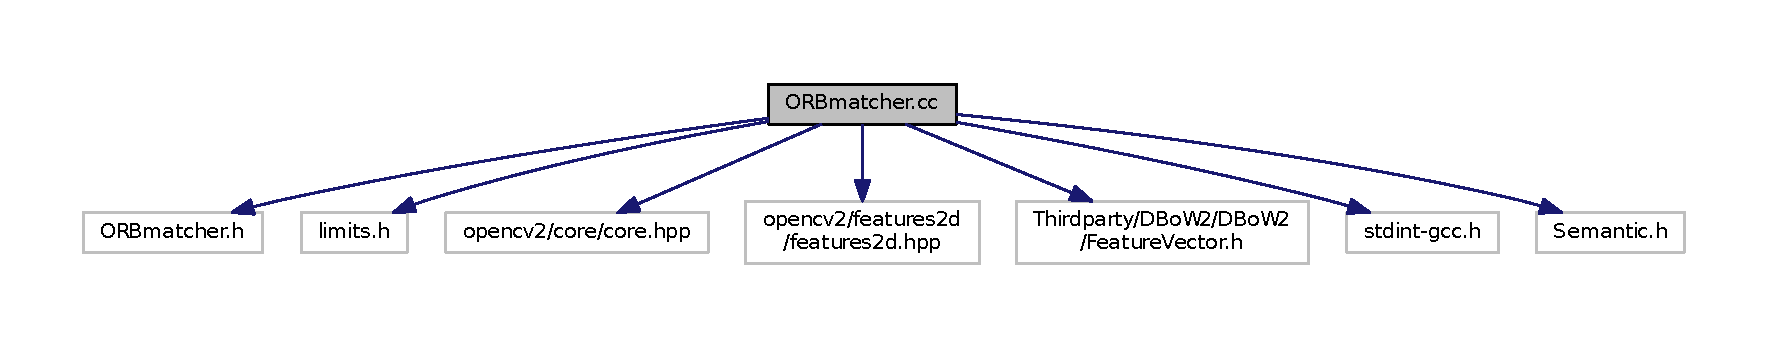
\includegraphics[width=350pt]{ORBmatcher_8cc__incl}
\end{center}
\end{figure}
\subsection*{Namespaces}
\begin{DoxyCompactItemize}
\item 
 \hyperlink{namespaceORB__SLAM2}{O\+R\+B\+\_\+\+S\+L\+A\+M2}
\end{DoxyCompactItemize}

\hypertarget{PnPsolver_8cc}{}\section{Pn\+Psolver.\+cc File Reference}
\label{PnPsolver_8cc}\index{Pn\+Psolver.\+cc@{Pn\+Psolver.\+cc}}
{\ttfamily \#include $<$iostream$>$}\\*
{\ttfamily \#include \char`\"{}Pn\+Psolver.\+h\char`\"{}}\\*
{\ttfamily \#include $<$vector$>$}\\*
{\ttfamily \#include $<$cmath$>$}\\*
{\ttfamily \#include $<$opencv2/core/core.\+hpp$>$}\\*
{\ttfamily \#include \char`\"{}Thirdparty/\+D\+Bo\+W2/\+D\+Utils/\+Random.\+h\char`\"{}}\\*
{\ttfamily \#include $<$algorithm$>$}\\*
Include dependency graph for Pn\+Psolver.\+cc\+:\nopagebreak
\begin{figure}[H]
\begin{center}
\leavevmode
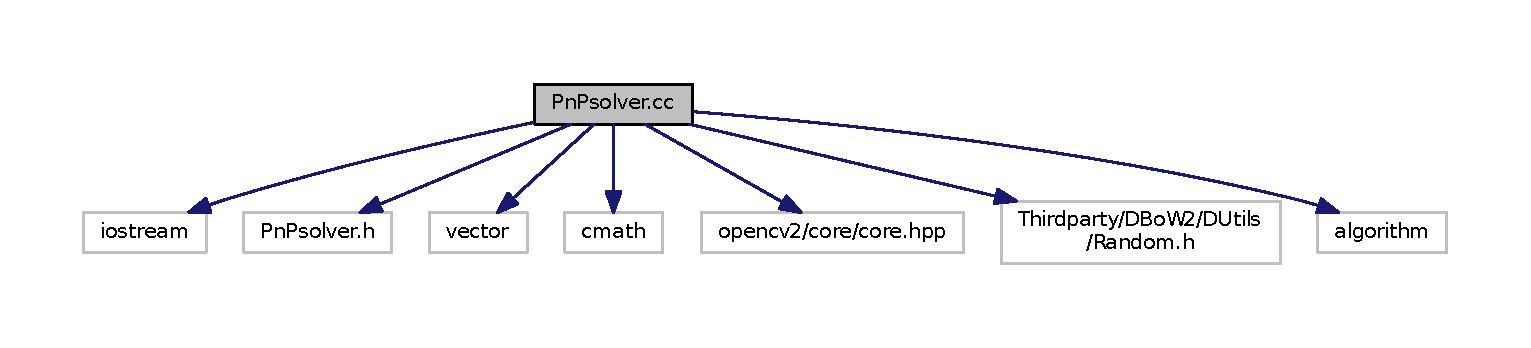
\includegraphics[width=350pt]{PnPsolver_8cc__incl}
\end{center}
\end{figure}
\subsection*{Namespaces}
\begin{DoxyCompactItemize}
\item 
 \hyperlink{namespaceORB__SLAM2}{O\+R\+B\+\_\+\+S\+L\+A\+M2}
\end{DoxyCompactItemize}

\hypertarget{RegionProps_8cc}{}\section{Region\+Props.\+cc File Reference}
\label{RegionProps_8cc}\index{Region\+Props.\+cc@{Region\+Props.\+cc}}
{\ttfamily \#include \char`\"{}regionprops.\+h\char`\"{}}\\*
{\ttfamily \#include $<$iostream$>$}\\*
Include dependency graph for Region\+Props.\+cc\+:\nopagebreak
\begin{figure}[H]
\begin{center}
\leavevmode
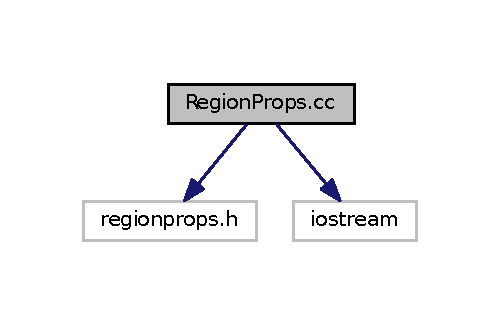
\includegraphics[width=240pt]{RegionProps_8cc__incl}
\end{center}
\end{figure}

\hypertarget{Semantic_8cc}{}\section{Semantic.\+cc File Reference}
\label{Semantic_8cc}\index{Semantic.\+cc@{Semantic.\+cc}}
{\ttfamily \#include \char`\"{}Semantic.\+h\char`\"{}}\\*
{\ttfamily \#include \char`\"{}Mask\+Net.\+h\char`\"{}}\\*
{\ttfamily \#include \char`\"{}Slam\+Config.\+h\char`\"{}}\\*
Include dependency graph for Semantic.\+cc\+:\nopagebreak
\begin{figure}[H]
\begin{center}
\leavevmode
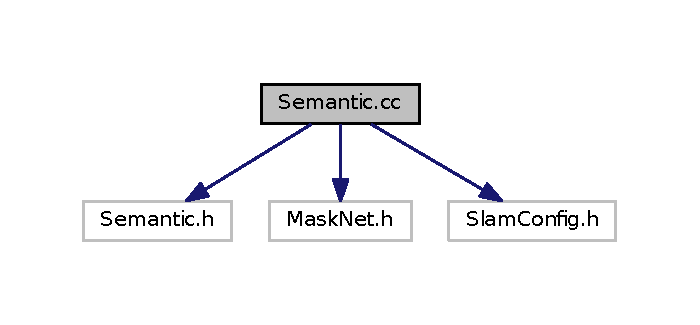
\includegraphics[width=336pt]{Semantic_8cc__incl}
\end{center}
\end{figure}
\subsection*{Namespaces}
\begin{DoxyCompactItemize}
\item 
 \hyperlink{namespaceORB__SLAM2}{O\+R\+B\+\_\+\+S\+L\+A\+M2}
\end{DoxyCompactItemize}
\subsection*{Macros}
\begin{DoxyCompactItemize}
\item 
\#define \hyperlink{Semantic_8cc_ad72dbcf6d0153db1b8d8a58001feed83}{D\+E\+B\+UG}~0
\end{DoxyCompactItemize}


\subsection{Macro Definition Documentation}
\index{Semantic.\+cc@{Semantic.\+cc}!D\+E\+B\+UG@{D\+E\+B\+UG}}
\index{D\+E\+B\+UG@{D\+E\+B\+UG}!Semantic.\+cc@{Semantic.\+cc}}
\subsubsection[{\texorpdfstring{D\+E\+B\+UG}{DEBUG}}]{\setlength{\rightskip}{0pt plus 5cm}\#define D\+E\+B\+UG~0}\hypertarget{Semantic_8cc_ad72dbcf6d0153db1b8d8a58001feed83}{}\label{Semantic_8cc_ad72dbcf6d0153db1b8d8a58001feed83}


Definition at line 11 of file Semantic.\+cc.


\hypertarget{Sim3Solver_8cc}{}\section{Sim3\+Solver.\+cc File Reference}
\label{Sim3Solver_8cc}\index{Sim3\+Solver.\+cc@{Sim3\+Solver.\+cc}}
{\ttfamily \#include \char`\"{}Sim3\+Solver.\+h\char`\"{}}\\*
{\ttfamily \#include $<$vector$>$}\\*
{\ttfamily \#include $<$cmath$>$}\\*
{\ttfamily \#include $<$opencv2/core/core.\+hpp$>$}\\*
{\ttfamily \#include \char`\"{}Key\+Frame.\+h\char`\"{}}\\*
{\ttfamily \#include \char`\"{}O\+R\+Bmatcher.\+h\char`\"{}}\\*
{\ttfamily \#include \char`\"{}Thirdparty/\+D\+Bo\+W2/\+D\+Utils/\+Random.\+h\char`\"{}}\\*
Include dependency graph for Sim3\+Solver.\+cc\+:\nopagebreak
\begin{figure}[H]
\begin{center}
\leavevmode
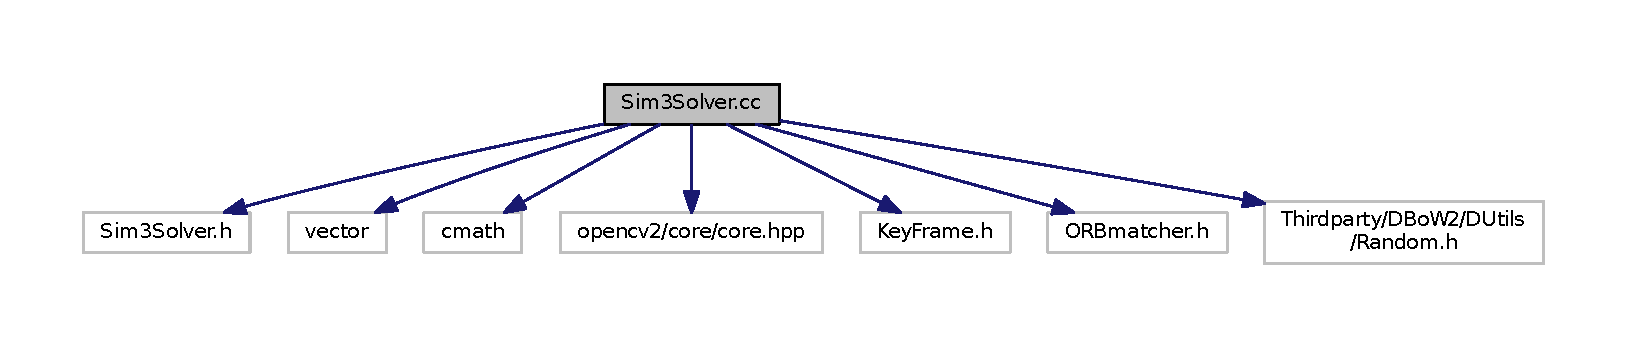
\includegraphics[width=350pt]{Sim3Solver_8cc__incl}
\end{center}
\end{figure}
\subsection*{Namespaces}
\begin{DoxyCompactItemize}
\item 
 \hyperlink{namespaceORB__SLAM2}{O\+R\+B\+\_\+\+S\+L\+A\+M2}
\end{DoxyCompactItemize}

\hypertarget{SlamConfig_8cc}{}\section{Slam\+Config.\+cc File Reference}
\label{SlamConfig_8cc}\index{Slam\+Config.\+cc@{Slam\+Config.\+cc}}
{\ttfamily \#include \char`\"{}Slam\+Config.\+h\char`\"{}}\\*
Include dependency graph for Slam\+Config.\+cc\+:\nopagebreak
\begin{figure}[H]
\begin{center}
\leavevmode
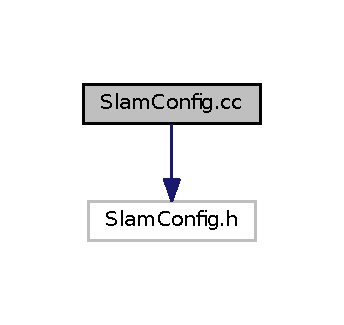
\includegraphics[width=165pt]{SlamConfig_8cc__incl}
\end{center}
\end{figure}
\subsection*{Namespaces}
\begin{DoxyCompactItemize}
\item 
 \hyperlink{namespaceORB__SLAM2}{O\+R\+B\+\_\+\+S\+L\+A\+M2}
\end{DoxyCompactItemize}

\hypertarget{System_8cc}{}\section{System.\+cc File Reference}
\label{System_8cc}\index{System.\+cc@{System.\+cc}}
{\ttfamily \#include \char`\"{}System.\+h\char`\"{}}\\*
{\ttfamily \#include \char`\"{}Converter.\+h\char`\"{}}\\*
{\ttfamily \#include $<$unistd.\+h$>$}\\*
{\ttfamily \#include $<$thread$>$}\\*
{\ttfamily \#include $<$pangolin/pangolin.\+h$>$}\\*
{\ttfamily \#include $<$iomanip$>$}\\*
Include dependency graph for System.\+cc\+:\nopagebreak
\begin{figure}[H]
\begin{center}
\leavevmode
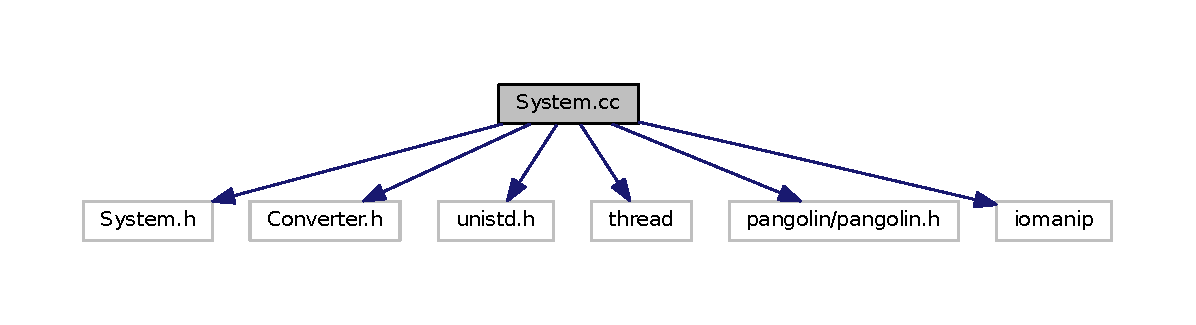
\includegraphics[width=350pt]{System_8cc__incl}
\end{center}
\end{figure}
\subsection*{Namespaces}
\begin{DoxyCompactItemize}
\item 
 \hyperlink{namespaceORB__SLAM2}{O\+R\+B\+\_\+\+S\+L\+A\+M2}
\end{DoxyCompactItemize}

\hypertarget{Tracking_8cc}{}\section{Tracking.\+cc File Reference}
\label{Tracking_8cc}\index{Tracking.\+cc@{Tracking.\+cc}}
{\ttfamily \#include \char`\"{}Tracking.\+h\char`\"{}}\\*
{\ttfamily \#include $<$opencv2/core/core.\+hpp$>$}\\*
{\ttfamily \#include $<$opencv2/features2d/features2d.\+hpp$>$}\\*
{\ttfamily \#include $<$unistd.\+h$>$}\\*
{\ttfamily \#include \char`\"{}Frame.\+h\char`\"{}}\\*
{\ttfamily \#include \char`\"{}O\+R\+Bmatcher.\+h\char`\"{}}\\*
{\ttfamily \#include \char`\"{}Frame\+Drawer.\+h\char`\"{}}\\*
{\ttfamily \#include \char`\"{}Converter.\+h\char`\"{}}\\*
{\ttfamily \#include \char`\"{}Map.\+h\char`\"{}}\\*
{\ttfamily \#include \char`\"{}Initializer.\+h\char`\"{}}\\*
{\ttfamily \#include \char`\"{}Optimizer.\+h\char`\"{}}\\*
{\ttfamily \#include \char`\"{}Pn\+Psolver.\+h\char`\"{}}\\*
{\ttfamily \#include $<$iostream$>$}\\*
{\ttfamily \#include $<$mutex$>$}\\*
{\ttfamily \#include \char`\"{}Semantic.\+h\char`\"{}}\\*
Include dependency graph for Tracking.\+cc\+:\nopagebreak
\begin{figure}[H]
\begin{center}
\leavevmode
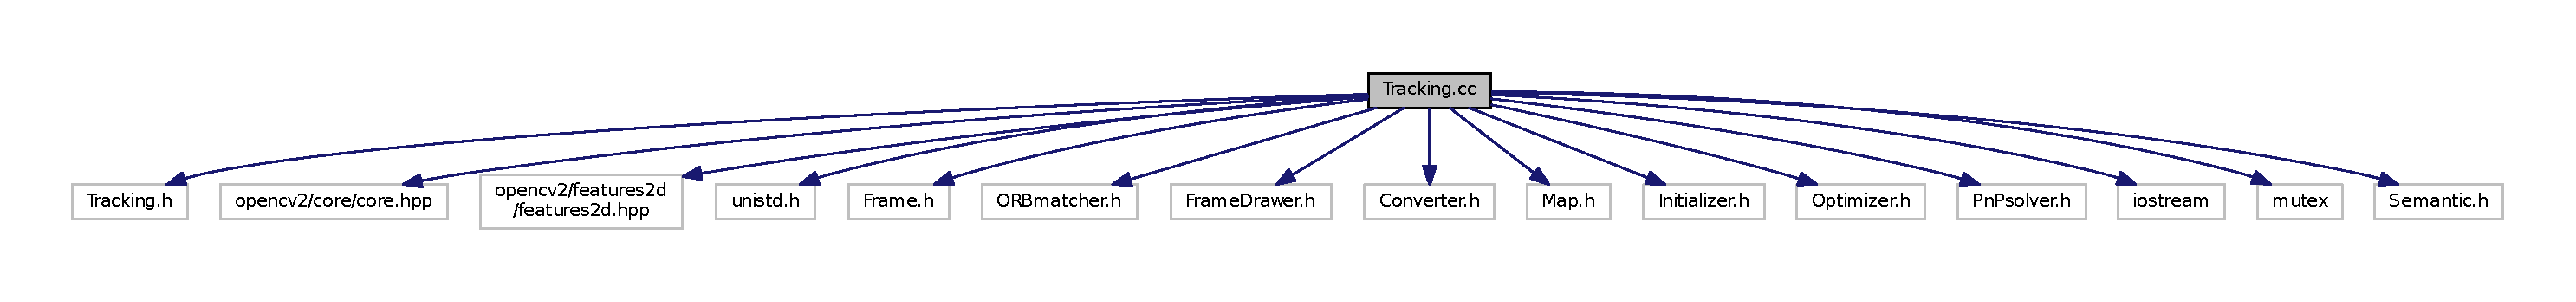
\includegraphics[width=350pt]{Tracking_8cc__incl}
\end{center}
\end{figure}
\subsection*{Namespaces}
\begin{DoxyCompactItemize}
\item 
 \hyperlink{namespaceORB__SLAM2}{O\+R\+B\+\_\+\+S\+L\+A\+M2}
\end{DoxyCompactItemize}

\hypertarget{Viewer_8cc}{}\section{Viewer.\+cc File Reference}
\label{Viewer_8cc}\index{Viewer.\+cc@{Viewer.\+cc}}
{\ttfamily \#include \char`\"{}Viewer.\+h\char`\"{}}\\*
{\ttfamily \#include $<$pangolin/pangolin.\+h$>$}\\*
{\ttfamily \#include $<$unistd.\+h$>$}\\*
{\ttfamily \#include $<$mutex$>$}\\*
Include dependency graph for Viewer.\+cc\+:\nopagebreak
\begin{figure}[H]
\begin{center}
\leavevmode
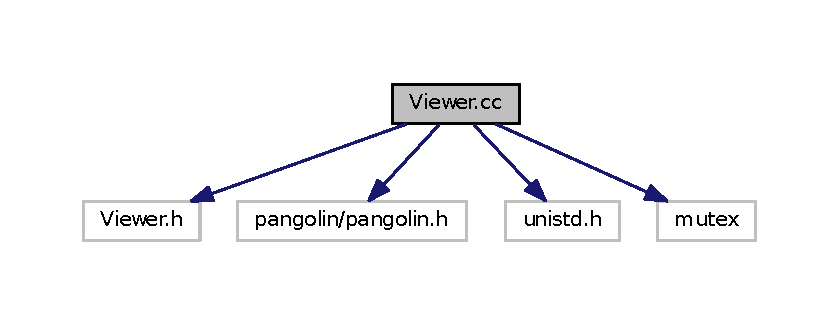
\includegraphics[width=350pt]{Viewer_8cc__incl}
\end{center}
\end{figure}
\subsection*{Namespaces}
\begin{DoxyCompactItemize}
\item 
 \hyperlink{namespaceORB__SLAM2}{O\+R\+B\+\_\+\+S\+L\+A\+M2}
\end{DoxyCompactItemize}

%--- End generated contents ---

% Index
\backmatter
\newpage
\phantomsection
\clearemptydoublepage
\addcontentsline{toc}{chapter}{Index}
\printindex

\end{document}
